%!TEX root = ../main.tex
\chapter{随机缓变粗糙表面光阴极的粗糙度热发射度}
\label{chap:roughness}

光阴极追求尽可能小的热发射度以及尽可能大的量子效率。D. Dowell 利用光电效应的三步模型给出了单光子光电效应光滑金属阴极体发射情形中,量子效率与发射度的公式:

\begin{eqnarray}
\text{QE}(\omega) &\approx& \dfrac{1-R(\omega)}{1+\dfrac{\lambda_{\text{opt}}}{\lambda_{e-e}(\omega)}}\frac{(\hbar\omega-\phi_{\text{eff}})^2}{8\phi_{\text{eff}}(E_F+\phi_{\text{eff}})}\label{eq:QE_d}\\
\varepsilon_{n,x} &=& \sigma_x\sqrt{\dfrac{\hbar\omega-\phi_{\text{eff}}}{3mc^2}}\label{eq:emit_d}
\end{eqnarray}

公式 \ref{eq:QE_d} 与 Cu 阴极的实验结果符合的相当好,但是公式 \ref{eq:emit_d} 却与各实验室的测量值出现了相当大的偏差。若采用 Cu 的文献逸出功 $\phi=4.65\,\text{eV}$,则各实验室的测量值均比公式预测值大 2 倍左右。一般猜测热发射度的增大是由光滑表面的假设失效导致的,也即热发射度中也包含了表面粗糙度的贡献。表面粗糙度对热发射度的贡献分成两种,一种是由于电子发射方向在粗糙表面的离散造成的热发射度,另一种是由阴极表面杂散电场造成的热发射度。对于计算粗糙度热发射度对总体热发射度的贡献,文献中往往采用二维模型或单频三维模型给出大概的量级,半定量地说明粗糙度对热发射度有较大贡献,但却无法和测量值做更精细的比较。因此粗糙度热发射度是否是发射度测量值大于理论值的唯一原因,尚无定论。

本章的目的就是较精确的计算三维粗糙表面粗糙度对热发射度的贡献,为此,需要精确计算激光入射后在粗糙表面产生的出射电子相空间分布。该分布可以利用光阴极的点扩散函数求出。需要注意的是,使用三步模型计算光电发射过程中,本文采取了和 Dowell 相似的假设,即体发射假设,因此本章给出的具体公式仅适用于体发射情形。但是利用点扩散函数来精确计算粗糙度对热发射度贡献的思路与发射模型无关,依然适用于表面发射等更广泛的情形。

\section{\label{s:psf}光阴极热发射度的点扩散函数}
当激光入射一个均匀 YAG 屏时,为了预测 YAG 屏上的图像,我们只需要知道激光的横向功率密度分布,以及激光单点入射时屏幕上的图像。后者就是 YAG 屏的点扩散函数(Point Spread Function,PSF)。点扩散函数本质上描述了 YAG 屏对于激光的冲击响应。假设屏幕的点扩散函数为 $f(x, y)$,激光横向功率密度分布为 $I(x, y)$,那么激光入射屏幕时的图像 $D(x, y)$ 就可写成二者的卷积:
\begin{equation}
D(x, y) = I(x, y) * f(x, y)
\label{eq:PSF}
\end{equation}

当我们考虑一个光阴极对入射激光的响应时,也可借鉴类似的概念,唯一的不同在于,光阴极对激光的响应是出射电子的相空间分布,即同时包含空间分布和动量分布;而屏幕对激光的响应是屏幕上的亮度分布,只是空间分布。若我们可以求出光阴极表面任意位置的点扩散函数(不同位置由于起伏可能点扩散函数不同),那么当我们知道入射激光的分布时,就可以直接通过卷积求出光阴极的出射电子相空间分布,从而计算出精确的发射度。下面我们从简单情形考虑,先计算正入射情形下的点扩散函数。

\subsection{正入射情形的光阴极点扩散函数}
为推导光阴极点扩散函数的解析形式,我们采用和 Dowell 相同的假设,即:体发射模型,阴极表面光滑,临界发射(即所有光电子在金属中无散射)。推导中所采用的坐标系统如图 \ref{fig:coor} 所示。

\begin{figure}[htbp]
\centering
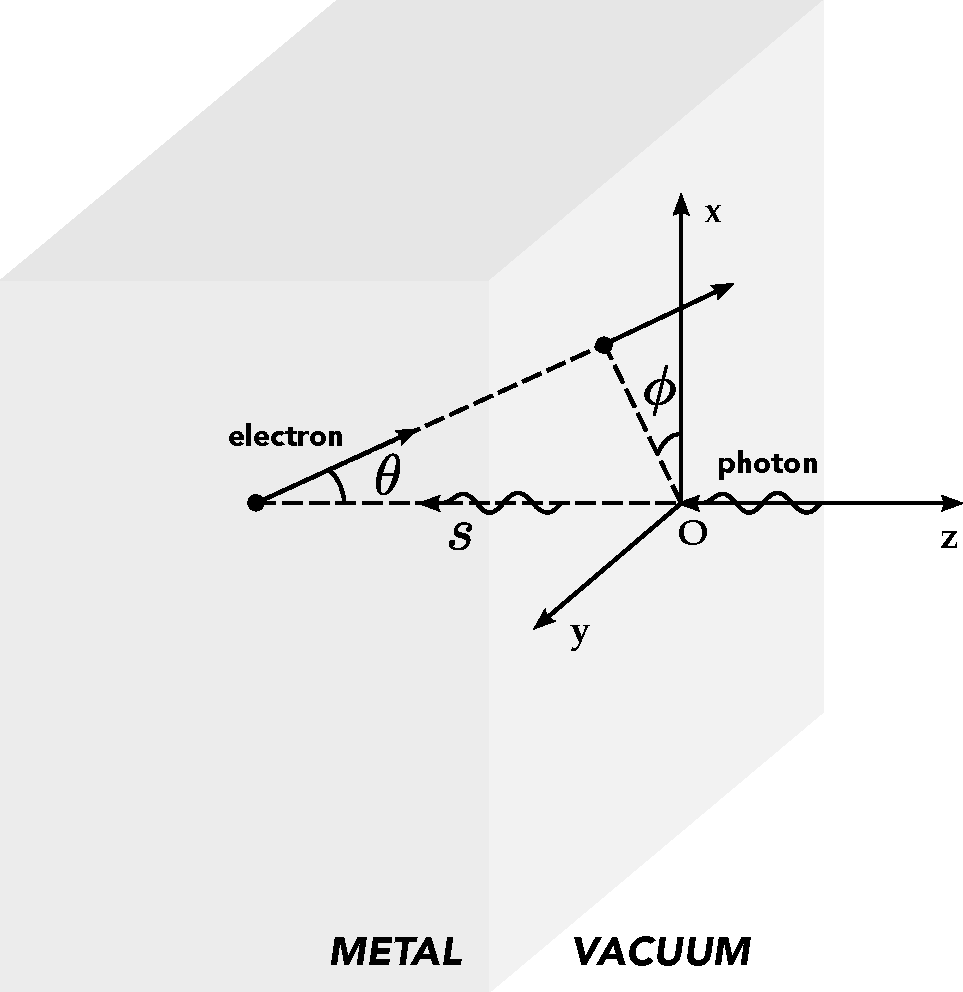
\includegraphics[width=0.5\textwidth]{coor}
\caption{\label{fig:coor} 单点正入射情形下光滑金属阴极体发射示意图,坐标和变量的定义请参见图中标注。}
\end{figure}

采用三步模型,我们可以获得一个正入射的光子入射阴极后,行进距离 $s$ 后被一个能量为 $E$ 的电子所吸收,随后该电子以空间角 $(\theta, \phi)$ 无散射出射并最终逃逸出金属表面成为光电子的概率密度。公式如式 \ref{eq:f} 所示。

\begin{eqnarray}
f(s, \theta, \phi, E, \omega) &=& (1-R)\dfrac{1}{\lambda_{\text{opt}}}\exp\left[-s\left(\dfrac{1}{\lambda_{\text{opt}}} + \dfrac{1}{\bar{\lambda}_{\text{e-e}}}\right)\right]\nonumber\\
&&\cdot\dfrac{H(E_\text{F}-E)H(E+\hbar\omega-E_\text{F})}{\hbar\omega}\dfrac{\sin\theta}{4\pi}
\label{eq:f}
\end{eqnarray}

式 \ref{eq:f} 中的 $H(x)$ 函数是 Heaviside 阶跃函数。为简化形式,令:
\begin{eqnarray}
\frac{1}{\lambda} &=& \frac{1}{\lambda_{\text{opt}}} + \frac{1}{\bar{\lambda}_{\text{e-e}}}\nonumber\\
C &=& \frac{1-R}{\lambda_{\text{opt}}\cdot 4\pi\hbar\omega}\\
p_m &=& \sqrt{2m(E_F+\phi_{\text{eff}})}\nonumber\\
p_M &=& \sqrt{2m(E_F+\hbar\omega)}\nonumber
\label{eq:pm}
\end{eqnarray}
考虑到两组坐标 $(s, \theta, \phi, E, \omega)$ 和 $(x, y, p_x, p_y, p_z)$ 之间的关系:
\begin{eqnarray}
x &=& s\tan\theta\cos\phi\nonumber\\
y &=& s\tan\theta\sin\phi \nonumber\\
p_x &=& \sqrt{2m(E+\hbar\omega)}\sin\theta\cos\phi\\
p_y &=& \sqrt{2m(E+\hbar\omega)}\sin\theta\sin\phi\nonumber\\
p_z &=& \sqrt{2m(E+\hbar\omega)\cos^2\theta - 2m(E_F+\phi_{\text{eff}})}\nonumber
\label{eq:trans}
\end{eqnarray}
我们可以尝试采用雅可比矩阵进行坐标变换。然而不幸的是,上面两组坐标系统并不是一一对应的,因此雅可比行列式为 0,也就是说,我们无法直接通过雅可比矩阵将两个坐标系下的概率分布建立连接。考虑到单点正入射情形时的出射电子相空间分布的轴对称性,采用一个中转坐标系 $(r, p_r, p_z)$ 可以达成连接的目的。

对 $f(s, \theta, \phi, E, \omega)$ 的 $\phi$ 进行积分,可以获得:$f(s,\theta,E;\omega) = 2\pi Ce^{-\frac{s}{\lambda}}\sin\theta$。之后令 $p=\sqrt{2m(E+\hbar\omega)}$,就可以建立起 $(s,\theta,E)$ 与 $(r, p_r, p_z)$ 之间的连接如下:
\begin{eqnarray}
r &=& s\tan\theta\nonumber\\
p_r &=& p\sin\theta\\
p_z &=& \sqrt{p^2-p_r^2-p_m^2}\nonumber
\label{eq:apatrans}
\end{eqnarray}
两坐标系统间的雅可比行列式为:
\begin{eqnarray}
|J| &=& \left|
\renewcommand{\arraystretch}{2.5}
\begin{array}{ccc}
0 & \dfrac{p_r}{m} & \dfrac{p_z}{m} \\
\dfrac{\sqrt{p_z^2+p_m^2}}{p_r} & -\dfrac{r\sqrt{p_z^2+p_m^2}}{p_r^2} & \dfrac{r}{p_r}\dfrac{p_z}{\sqrt{p_z^2+p_m^2}} \\
0 & \dfrac{\sqrt{p_z^2+p_m^2}}{p_r^2+p_z^2+p_m^2} & -\dfrac{p_rp_z}{\sqrt{p_z^2+p_m^2}(p_r^2+p_z^2+p_m^2)}
\end{array} \right|\nonumber\\
&=& \dfrac{1}{m}\cdot\dfrac{p_z}{p_r}
\end{eqnarray}
于是 $dEdsd\theta = |J|drdp_rdp_z$。进而有 $(r, p_r, p_z)$ 坐标系下的点扩散函数:
\begin{eqnarray}
f(r, p_r, p_z)&=&C\exp\left[-\dfrac{\sqrt{p_z^2+p_m^2}}{p_r}\cdot\dfrac{r}{\lambda}\right]\cdot\dfrac{p_z}{\sqrt{p_r^2+p_z^2+p_m^2}}\nonumber\\
&&\cdot H(p_r)H(p_z)H(r)H(p_M^2-p_m^2-p_r^2-p_z^2)
\end{eqnarray}

现在我们要利用电子相空间分布的轴对称性来将 $(r, p_r, p_z)$ 下的点扩散函数变换到 $(x, y, p_x, p_y, p_z)$ 坐标系中。假定 $(x, y, p_x, p_y, p_z)$ 坐标系下的点扩散函数有下面的一般形式:
\begin{equation}
f(x, y, p_x, p_y, p_z) = g(r, p_r, p_z)\delta(xp_y-yp_x)H(xp_x)
\label{eq:apa_general}
\end{equation}
利用积分恒等关系:
\begin{equation}
dp_z\iint_{p_r}^{p_r+dp_r}\!\!\!dp_x\,dp_y\iint_{r}^{r+dr}\!\!\!dx\,dy\,f(x, y, p_x, p_y, p_z) = f(r, p_r, p_z)\,dr\,dp_r\,dp_z
\end{equation}
可获得 $g(r, p_r, p_z)$ 与 $f(r, p_r, p_z)$ 的关系:
\[
g(r, p_r, p_z) = \dfrac{1}{2\pi}f(r, p_r, p_z)
\]
代入 $r = \sqrt{x^2+y^2}$ 和 $p_r = \sqrt{p_x^2+p_y^2}$ 到式 \ref{eq:apa_general},我们就获得了光阴极的正入射点扩散函数,如式 \ref{eq:psf} 所示。

\begin{eqnarray}
f(x, y, p_x, p_y, p_z)&=&C\exp\left[-\dfrac{\sqrt{p_z^2+p_m^2}}{\sqrt{p_x^2+p_y^2}}\cdot\dfrac{\sqrt{x^2+y^2}}{\lambda}\right]\cdot\dfrac{p_z}{\sqrt{p_x^2+p_y^2+p_z^2+p_m^2}}\cdot \delta(xp_y-yp_x)\nonumber\\
&&\cdot H(p_z)H(xp_x)H(p_M^2-p_m^2-p_x^2-p_y^2-p_z^2)
\label{eq:psf}
\end{eqnarray}

利用式 \ref{eq:psf} 所示的点扩散函数,我们可以精确计算任意横向功率密度分布的激光正入射光滑光阴极后的光电子相空间分布。例如,一个横向高斯分布的激光:
\[
I(x, y) = \dfrac{I_0}{2\pi\sigma_x\sigma_y}\cdot\exp\left[-\left(\dfrac{x^2}{2\sigma_x^2}+\dfrac{y^2}{2\sigma_y^2}\right)\right]
\]
所激发的光电子相空间分布 $G(\bm{x},\bm{p})$ 如式 \ref{eq:guass} 所示。
\begin{eqnarray}
G &=& \dfrac{\sqrt{\pi}}{2}\dfrac{1}{\sqrt{\dfrac{p_x^2}{2\sigma_x^2}+\dfrac{p_y^2}{2\sigma_y^2}}}\exp\left[-\dfrac{x^2}{2\sigma_x^2}-\dfrac{y^2}{2\sigma_y^2}+T^2\right]\cdot\text{erfc}(T)\nonumber\\
T &=& \dfrac{-\dfrac{xp_x}{2\sigma_x^2}-\dfrac{yp_y}{2\sigma_y^2}+\dfrac{\sqrt{p_z^2+p_m^2}}{2\lambda}}{\sqrt{\dfrac{p_x^2}{2\sigma_x^2}+\dfrac{p_y^2}{2\sigma_y^2}}}
\label{eq:guass}
\end{eqnarray}

\subsection{\label{ss:dowell}对 Dowell 发射度公式的修正}
统计意义下的发射度定义如下:
\begin{equation}
\varepsilon_{D,x}^2 = \langle x^2\rangle_D\langle p_x^2\rangle_D-\langle xp_x\rangle_D^2
\label{eq:emit_def}
\end{equation}
式 \ref{eq:emit_def} 中的符号 D 代表电子相空间分布。在 Dowell 发射度公式的推导中,$\langle xp_x\rangle$ 所代表的交叉项被忽略掉了,理由是假设电子动量分布与光子入射位置相互独立。Dowell 同时假定了出射光电子的横向空间分布与入射激光的横向分布相同。若这些假设成立,则统计意义的发射度计算就可以简化为 $\varepsilon_{x} = \sqrt{\langle x^2\rangle\langle p_x^2\rangle}=\sigma_x\sqrt{\langle p_x^2\rangle}$,因此 $\varepsilon_{x,n} = \sigma_x\cdot\Delta_x$,其中 $\Delta_x$ 被称做归一化散角(有时也称为归一化热发射度),定义为 $\sqrt{\langle p_x^2\rangle}/mc$。利用我们前面推导的点扩散函数,通过计算式 \ref{eq:emit_def} 中的各统计项,可以检验 Dowell 发射度公式的精确程度。

假设我们有一个形式为 $v(x,y,p_x,p_y,p_z)$ 的变量 $v$,为了计算 $v$ 在概率密度分布 $D=I*f$ 下的期望,我们有式 \ref{eq:stat} 中所展示的规律:
\begin{equation}
\langle v \rangle_{D} = \langle v\rangle_{I * f} = \langle v(x_I+x_f, y_I+y_f, p_x, p_y, p_z)\rangle_{I\cdot f}
\label{eq:stat}
\end{equation}
式 \ref{eq:stat} 中有下标的 $x$ 或 $y$ 代表它们仅在下标所示的分布中是变量,而在其他分布中是常数。例如当计算 $\langle x_I\rangle_{f}$ 时 $x_I$ 是个常数,而当计算 $\langle x_I\rangle_{I}$ 时则是变量。 同时约定 $\langle\cdots\rangle_{I\cdot f}$ 代表求复合平均 $\langle\langle\cdots\rangle_{I}\rangle_{f}$ 或者 $\langle\langle\cdots\rangle_{f}\rangle_{I}$。由于交换内外括号的下标并不会改变统计结果,我们可以将复合平均符号写做 $\langle\cdots\rangle_{I\cdot f}$。

经过代数计算,最终可获得:
\begin{eqnarray}
\varepsilon_{D, x}^2 &=& \langle x^2\rangle_I\langle p_x^2\rangle_f+\varepsilon_f^2
\label{eq:emit_acc}
\end{eqnarray}
其中 $\varepsilon_f^2$ 代表单点入射发射度,即 $\langle x^2\rangle_f\langle p_x^2\rangle_f-\langle xp_x\rangle_f^2$。式 \ref{eq:emit_acc} 右侧第一项就是 Dowell 给出的发射度公式,所以第二项 $\varepsilon_f$ 就是 Dowell 发射度公式的误差。当 $\hbar\omega$ 接近 $\phi_{\text{eff}}$ 时(也即临界发射,这也是一般光阴极采用的工作状态)。下面我们尝试计算 $\varepsilon_f$。至少有两种方式计算单点热发射度,即 1)直接使用式 \ref{eq:psf} 和 2)采用原始的概率密度公式 \ref{eq:f}。下面使用对人类更友好的第二种方式进行计算。

简化起见,令 $p = \sqrt{2m(E+\hbar\omega)}$ 以及 $\cos\theta_M=p_m/p_M$,也令 $\Delta=p_M-p_m$ 以及 $\delta=(p_M-p_m)/p_m$。应用式 \ref{eq:f},我们有:
\begin{eqnarray*}
\langle x^2\rangle_f &=& \dfrac{\int_{p_m}^{p_M} pdp\int_0^{\infty} ds\int_0^{2\pi}d\phi\int_0^{\theta_M}d\theta (s\tan\theta\cos\phi)^2e^{-\frac{s}{\lambda}}\sin\theta}{\int_{p_m}^{p_M} pdp\int_0^{\infty} ds\int_0^{2\pi}d\phi\int_0^{\theta_M}d\theta e^{-\frac{s}{\lambda}}\sin\theta}\\
&=& \dfrac{\int_{p_m}^{p_M} pdp\int_0^{\infty} s^2e^{-\frac{s}{\lambda}}ds\int_0^{2\pi}\cos^2\phi d\phi\int_0^{\theta_M}\tan^2\theta\sin\theta d\theta}{\int_{p_m}^{p_M} pdp\int_0^{\infty} e^{-\frac{s}{\lambda}}ds\int_0^{2\pi}d\phi\int_0^{\theta_M}\sin\theta d\theta}\\
&=& \dfrac{\int_{p_m}^{p_M}pdp\cdot\lambda^3\Gamma(3)\cdot\pi\cdot(p/p_m+p_m/p-2)}{\int_{p_m}^{p_M}pdp\cdot\lambda\Gamma(1)\cdot2\pi\cdot(1-p_m/p)}\\
&=& \frac{\lambda^2}{p_m}\cdot\dfrac{\Delta^3/3}{\Delta^2/2} = \frac{2}{3}\lambda^2\delta
\end{eqnarray*}

\begin{eqnarray*}
\langle p_x^2\rangle_f &=& \dfrac{\int_{p_m}^{p_M} pdp\int_0^{\infty} ds\int_0^{2\pi}d\phi\int_0^{\theta_M}d\theta (p\sin\theta\cos\phi)^2e^{-\frac{s}{\lambda}}\sin\theta}{\int_{p_m}^{p_M} pdp\int_0^{\infty} ds\int_0^{2\pi}d\phi\int_0^{\theta_M}d\theta e^{-\frac{s}{\lambda}}\sin\theta}\\
&=& \dfrac{\int_{p_m}^{p_M} p^3dp\int_0^{\infty} e^{-\frac{s}{\lambda}}ds\int_0^{2\pi}\cos^2\phi d\phi\int_0^{\theta_M}\sin^3\theta d\theta}{\int_{p_m}^{p_M} pdp\int_0^{\infty} e^{-\frac{s}{\lambda}}ds\int_0^{2\pi}d\phi\int_0^{\theta_M}\sin\theta d\theta}\\
&=& \dfrac{\int_{p_m}^{p_M}p^3dp\cdot\lambda\Gamma(1)\cdot\pi\cdot(2/3-p_m/p+1/3\cdot p_m^3/p^3)}{\int_{p_m}^{p_M}pdp\cdot\lambda\Gamma(1)\cdot2\pi\cdot(1-p_m/p)}\\
&=& \frac{1}{2}\cdot\dfrac{\Delta^4/6+p_m\cdot\Delta^3/3}{\Delta^2/2} = \frac{1}{6}\Delta(\Delta+2p_m)
\end{eqnarray*}

\begin{eqnarray*}
\langle xp_x\rangle_f &=& \dfrac{\int_{p_m}^{p_M} pdp\int_0^{\infty} ds\int_0^{2\pi}d\phi\int_0^{\theta_M}d\theta (sp\tan\theta\sin\theta\cos^2\phi)e^{-\frac{s}{\lambda}}\sin\theta}{\int_{p_m}^{p_M} pdp\int_0^{\infty} ds\int_0^{2\pi}d\phi\int_0^{\theta_M}d\theta e^{-\frac{s}{\lambda}}\sin\theta}\\
&=& \dfrac{\int_{p_m}^{p_M} p^2dp\int_0^{\infty} se^{-\frac{s}{\lambda}}ds\int_0^{2\pi}\cos^2\phi d\phi\int_0^{\theta_M}\tan\theta\sin^2\theta d\theta}{\int_{p_m}^{p_M} pdp\int_0^{\infty} e^{-\frac{s}{\lambda}}ds\int_0^{2\pi}d\phi\int_0^{\theta_M}\sin\theta d\theta}\\
&=& \dfrac{\int_{p_m}^{p_M}p^2dp\cdot\lambda^2\Gamma(2)\cdot\pi\cdot(-1/2-\ln(p_m/p)+1/2\cdot p_m^2/p^2)}{\int_{p_m}^{p_M}pdp\cdot\lambda\Gamma(1)\cdot2\pi\cdot(1-p_m/p)}\\
&=& \frac{\lambda}{2}\cdot\dfrac{\frac{1}{3}p_M^3\ln(p_M/p_m)-\frac{1}{9}(p_M^3-p_m^3)-\frac{1}{6}\Delta^2(p_M+2p_m)}{\Delta^2/2}\\
&=& \frac{1}{3}\lambda \Delta\left(1+\frac{1}{4}\delta+O(\delta^2)\right)\approx\frac{1}{3}\lambda \Delta
\end{eqnarray*}

把上面的计算结果带回统计意义发射度公式,就有:
\begin{eqnarray*}
\varepsilon_f &=& \sqrt{\langle x^2\rangle_f\langle p_x^2\rangle_f-\langle xp_x\rangle_f^2} \approx \frac{1}{3}\lambda\sqrt{\delta\cdot\Delta(\Delta+2p_m)-\Delta^2}\\
&=& \frac{1}{3}\lambda\sqrt{\delta\cdot\Delta^2+2\Delta^2-\Delta^2} = \frac{1}{3}\lambda\sqrt{\Delta^2\cdot(1+\delta)}\\
&\approx& \frac{1}{3}\lambda\Delta = \dfrac{1}{3}\lambda(p_M-p_m)
\end{eqnarray*}
也即 $\varepsilon_f$ 具有下面的近似形式:
\[
\varepsilon_f \approx \dfrac{1}{3}\lambda(p_M-p_m)
\]
其中 $p_M,p_m$ 和 $\lambda$ 与 式 \ref{eq:pm} 中的定义相同。而 $\langle p_x^2\rangle_f$ 可以写成:
\[
\langle p_x^2\rangle_f = \dfrac{1}{6}(p_M^2-p_m^2)
\]
取一阶近似,则修正后的发射度公式的近似形式就如下式所示:
\begin{equation}
\varepsilon_{D,x}^2 \approx \varepsilon_{\text{Dowell}}^2\left[1+\left(\dfrac{\lambda}{\sigma_x}\right)^2\cdot\dfrac{\delta}{3}\right]
\label{eq:emit_de}
\end{equation}
其中 $\delta = (p_M-p_m)/p_m$。代入表 \ref{tab:exp} 中所示的一组典型的实验参数,就有:
\[
\varepsilon_{D,x}^2 = \varepsilon_{\text{Dowell}}^2\left[1+\left(\dfrac{0.40\,\text{nm}}{\sigma_x}\right)^2\right]
\]

由于 $\sigma_x$ 的典型值在 100\,$\mu$m 量级,从上式可以看出,绝大多数情形下,Dowell 公式足够精确,在发射度计算中可以忽略动量分布与入射位置间的关系。

\begin{table}[htbp]
\caption{\label{tab:exp}
一组典型的光阴极物理参数。}
\centering
\begin{tabular}{llll}
\toprule
参数 & 值 & 单位 & 描述 \\
\midrule
$E_F$ & 7.0 & eV & Cu 的费米能级 \\
$\hbar\omega$ & 4.66 & eV & 光子能量 \\
$\phi_w$ & 4.31 & eV & Cu 的逸出功 \\
$E_{\text{rf}}$ & 50.0 & MV/m & 阴极表面电场强度 \\
$\lambda_{\text{opt}}$ & 12.58 & nm & Cu 中光子的平均自由程 \\
$\bar{\lambda}_{\text{e-e}}$ & 6.13 & nm & Cu 中电子的平均自由程 \\
\bottomrule
\end{tabular}
\end{table}

\subsection{\label{ss:approx}光电子相空间分布的近似形式}
从小节 \ref{ss:dowell} 中证明了一般情况下忽略电子动量分布与光子入射位置之间的关系是合理的,事实上这个结论可以从点扩散函数的观点直接得到。

考虑阴极表面点 \textbf{P}$(x_0, y_0)$ 附近的光电子相空间分布。利用式 \ref{eq:psf} 中给出的点扩散函数,容易证明点扩散函数的 rms 半径在亚纳米量级,且点扩散函数的幅度在 rms 半径外的区域迅速衰减到 0。因此我们定义以 \textbf{P} 点为中心 rms 半径为半径的圆形区域为有效区域。由于有效区域非常小,可以假设激光功率密度在 \textbf{P} 点的有效区域内基本为常数。同时对于有效区域外的被照射表面,其发射电子对点 \textbf{P} 处光电子相空间的贡献基本可以忽略。根据以上分析,点 \textbf{P} 处的光电子相空间分布可以近似如下:
\begin{eqnarray}
D\big|_{\textbf{P}} &=& I(x,y)*f(x,y,p_x,p_y,p_z)\big|_{x=x_0,y=y_0}\nonumber\\
&\approx& I(x_0,y_0)*f(x,y,p_x,p_y,p_z)\big|_{(x, y)\text{ in effective area}}\nonumber\\
&\approx& I(x_0,y_0)*f(x,y,p_x,p_y,p_z)\big|_{(x, y)\text{ in entire area}}\nonumber\\
&=& I(x_0,y_0)\cdot\iint dxdyf(x,y,p_x,p_y,p_z)\nonumber\\
&=& I(x_0,y_0)f_p(p_x,p_y,p_z)
\label{eq:approx}
\end{eqnarray}
上式就验证了前面的结论。

式 \ref{eq:approx} 中的函数 $f_p(p_x, p_y, p_z)$ 是动量点扩散函数,它描述了单点入射情形下的光电子动量空间分布。正如式 \ref{eq:approx} 所示,$f_p$ 就是 $f$ 对整个实空间 $(x, y)$ 的积分,因此可以计算得到动量点扩散函数的形式如下:
\begin{eqnarray}
f_p(p_x,p_y,p_z) &=& \dfrac{C_p p_z}{\sqrt{{p_z}^2+p_m^2}\cdot\sqrt{{p_x}^2+{p_y}^2+{p_z}^2+{p_m}^2}}\nonumber\\
&&\cdot H(p_z)H(p_M^2-p_m^2-p_x^2-p_y^2-p_z^2)
\label{eq:ppsf}
\end{eqnarray}
其中 $C_p$ 满足:
\[
C_p = \dfrac{1-R}{1+\dfrac{\lambda_{\text{opt}}}{\lambda_{e-e}}}\cdot\dfrac{1}{4\pi m\hbar\omega}
\]
近似形式的光电子分布函数将会在接下来的一般表面粗糙度热发射度计算中起到关键作用。

\section{\label{s:ana}随机缓变粗糙表面光阴极的粗糙度热发射度}
采用点扩散函数的独特好处在于,它可以处理真实场景下几乎任意表面形态的光阴极的热发射度。这里强调真实场景,是因为真实的光阴极通常是经过精细加工与打磨的,其表面在宏观上非常接近一个平面;但是从微观上看,加工过程中的车铣会在其表面留下较规则的条纹,其横向尺度一般在十几微米,起伏在百纳米级别,而打磨时会在阴极表面留下非常细小的起伏,其横向和纵向尺度一般在百纳米到纳米量级。尽管真实阴极表面会存在这些不均匀的形态,但其总体上依然是一个相当平滑的平面,我们称这种表面为随机缓变粗糙表面。

\subsection{缓变粗糙表面}
图 \ref{fig:rough} 展示了白光干涉仪下的一块真实阴极的表面形态。
\begin{figure}[htbp]
\centering
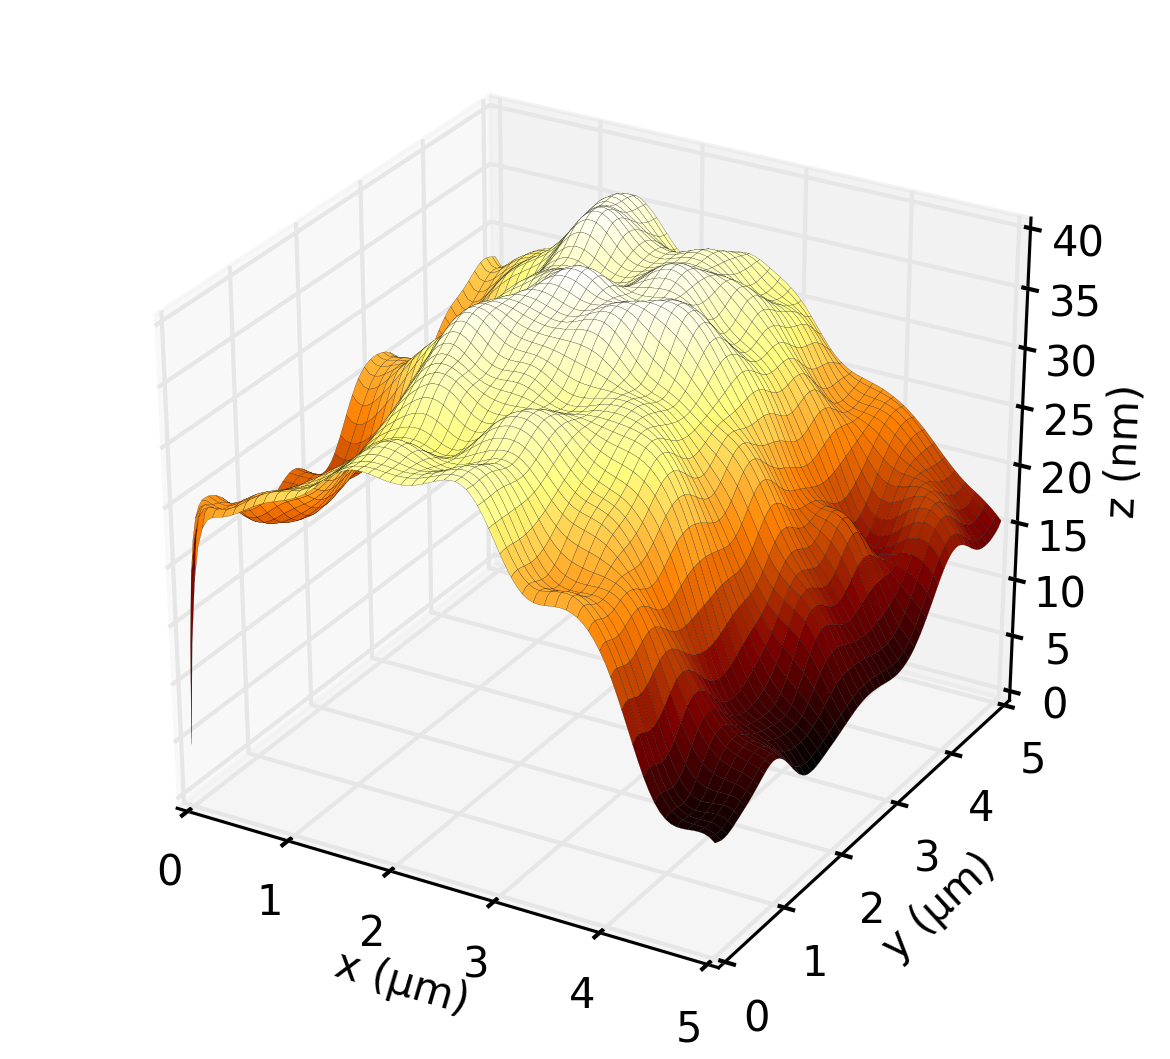
\includegraphics[width=0.6\textwidth]{surface}
\caption{\label{fig:rough} 白光干涉仪下一块真实阴极的表面形态。注意横纵坐标的单位不同。}
\end{figure}

人们通常使用振幅 $a$ 与空间周期 $\lambda$(或空间波数 $k$)来描述粗糙度的某个特定空间频率的分量。如前所述,一块经过抛光的阴极上通常存在两种粗糙度,即宏观粗糙度 $r_M$ 与微观粗糙度 $r_m$。这两种粗糙度的典型参数见表 \ref{tab:rough}。

\begin{table}[htbp]
\caption{\label{tab:rough}
粗糙度参数的典型值。}
\centering
\begin{tabular}{llll}
\toprule
参数 & 值 & 单位 & 描述 \\
\midrule
$a_m$ & 4 & nm & 微观粗糙度典型振幅 \\
$\lambda_m$ & 200 & nm & 微观粗糙度典型空间周期 \\
$a_M$ & 100 & nm & 宏观粗糙度典型振幅 \\
$\lambda_M$ & 16 & $\mu$m & 宏观粗糙度典型空间周期 \\
\bottomrule
\end{tabular}
\end{table}

缓变粗糙表面很难严格界定,因为不同情形下对缓变和粗糙的定义不同。但在光阴极领域,我们可以认为缓变粗糙表面有下面特征:其大部分空间分量的梯度都远小于 1。根据这个特点,定义某方向 $x$ 的缓变粗糙表面为满足下面条件的表面:
\begin{equation}
\text{rms}(R)\cdot\text{rms}(k_x) \ll 1
\label{eq:def_gus}
\end{equation}
其中 $k_x$ 是 $x$ 方向的空间波数, $R$ 是待考虑表面的振幅。 

这个定义其实是保证对于所有 $k \le k_{\max}$,$k\cdot R(x, y) \ll 1$。这里 $k_{\max}$ 我们所考虑的最大空间波数,因为对于 $k > k_{\max}$ 的空间分量,其振幅已经小到可以在计算粗糙度热发射度时忽略不计。我们以图 \ref{fig:conf} 所示的真实阴极表面为例,其空间频谱见图 \ref{fig:spec}。对该粗糙阴极表面计算得到各统计值如下:$\text{rms}(k_x)=3.45\,\mu\text{m}^{-1}, \text{rms}(R)=22.65\,\text{nm}$,因此 $\text{rms}(R)\cdot\text{rms}(k_x) = 0.08 \ll 1$。从频谱的强度分布可以看出,我们所关心的最大波数 $k_{x, \max}\sim 4\,\mu\text{m}^{-1}$(因为大部分的空间分量的能量都集中在这个区域内)。对于这个表面,容易看出 $\text{rms}(k_x)\sim k_{x, \max}$ 并且 $R(x, y)\sim\text{rms}(R)$,因此我们的定义式 \ref{eq:def_gus} 可以保证对于所有 $k \le k_{\max}$ 都有 $k\cdot R(x, y) \ll 1$。

本章接下来所有的讨论和推导都仅限于这种缓变粗糙表面。
%Paper~[5] assumed the surface morphology obey the form:
%\[ 
%R(x, y)=h\cos(kx)\cos(ky)
%\]which described a quasi-monochrome roughness, to derive the analytical formation of the roughness emittance. The result of paper~[5] showed that: $\varepsilon_{\text{roughness}}\propto \xi$, $\xi=hk$.

\subsection{\label{ss:gmpsf}推广的动量点扩散函数}

\begin{figure}[htbp]
\centering
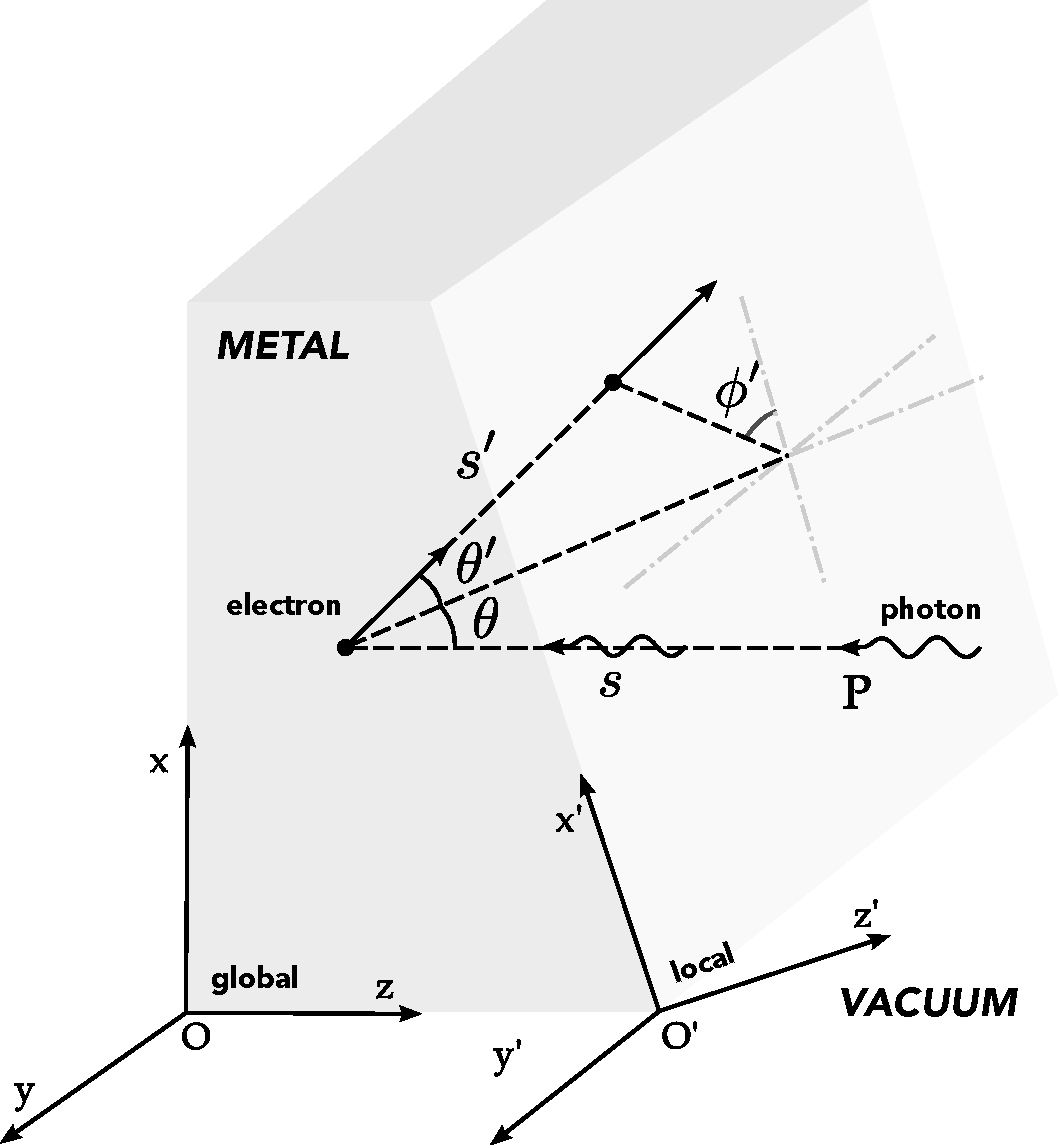
\includegraphics[width=0.5\textwidth]{coor2}
\caption{\label{fig:coor_m} 粗糙阴极表面某局部的体发射示意图。坐标系统和变量定义如图中标注所示。光滑和粗糙阴极的主要区别在于,对于粗糙阴极而言,激光基本上在表面任何一点都是(相对于该处法向)斜入射的。如图所示,一个光子以 $\theta$ 的入射角入射,在行进 $s$ 距离后,光子被一个电子吸收,随后电子向粗糙表面运动并成功逃逸处金属表面成为光电子。很明显斜入射时光电子发射的中心点不再是光子入射点 \textbf{P},而是距离点 \textbf{P} 有一个小的偏移。}
\end{figure}

当一束激光正入射一个表面形态函数为 $R(x, y)$ 的粗糙表面时,我们跟踪其中一个光子来看看中间的物理过程。假定该光子从阴极表面 \textbf{P}$(x_0, y_0)$ 点入射,由于点 \textbf{P} 的法向相对于全局坐标系的 z 轴存在一个夹角,光电发射过程除了发射中心不再是入射点外,其他几乎与光滑平面阴极的情形没有区别。

采用点扩散函数的观点来考虑上面的进程,我们可以采用和小节 \ref{ss:approx} 类似的想法。点 \textbf{P} 的邻域 $\Delta$ 可以看成一个法向相对于 $z$ 轴成一个夹角 $\theta$ 的平面,且激光功率密度在有效区域内近似常量 $I(x_0, y_0)$。为获得全局坐标系 $S$ 下的光电子相空间分布,可以首先获取局部坐标系 $S^{\prime}$(法向与全局坐标系 $z$ 轴成 $\theta$ 的夹角)下的光电子相空间分布 $D^{\prime}$,随后旋转 $D^{\prime}$ 到全局坐标系,进而获得 $D$。

为实现上面的想法,有必要将原始的正入射动量点扩散函数推广到一般入射情形。通过一定的计算,得到推广的动量点扩散函数如式 \ref{eq:g-ppsf} 所示。

\begin{eqnarray}
f_p(p_x,p_y,p_z) &=& \dfrac{C_p(\theta)p_z}{\sqrt{p_z^2+p_m^2}\cdot\sqrt{p_x^2+p_y^2+p_z^2+p_m^2}}\label{eq:g-ppsf}\\
C_p(\theta) &=& \dfrac{1-R(\theta)}{1+\dfrac{\lambda_{\text{opt}}}{\lambda_{e-e}}\cos\theta}\cdot\dfrac{1}{4\pi m\hbar\omega}\nonumber
\end{eqnarray}
为了使公式清晰我们省略了 Heaviside 阶跃函数。结合式 \ref{eq:approx} 和 \ref{eq:g-ppsf},获得局部坐标系下的光电子相空间分布:
\begin{equation}
D^{\prime}(x, y, p_x, p_y, p_z) = I(x_0,y_0)\cos\theta f_p(p_x, p_y, p_z)
\label{eq:l-dist}
\end{equation}

下一步是利用局部坐标系到全局坐标系的旋转矩阵将局部坐标系下光电子相空间分布变换到全局坐标系下。
将式 \ref{eq:g-ppsf} 代入式 \ref{eq:l-dist} 可以获得全局坐标系下分布的形式:
\begin{equation}
D^{\prime}= I(x_0,y_0)\cos\theta \dfrac{Cp_z^{\prime}}{\sqrt{{p_z^{\prime}}^2+p_m^2}\cdot\sqrt{{p_x^{\prime}}^2+{p_y^{\prime}}^2+{p_z^{\prime}}^2+p_m^2}}
\label{eq:apc_l2d}
\end{equation}
设局部与全局坐标系之间的变换矩阵为:
\begin{equation}
\mathbf{D}=\left(
\begin{array}{c}
\mathbf{m}\\
\mathbf{n}\\
\mathbf{k}
\end{array} \right)
\end{equation}
那么:
\begin{equation}
\mathbf{D}\cdot\left(
\begin{array}{c}
p_x\\
p_y\\
p_z
\end{array} \right)=\left(
\begin{array}{c}
p_x^{\prime}\\
p_y^{\prime}\\
p_z^{\prime}
\end{array} \right)
\label{eq:apc_trans}
\end{equation}
我们未指定 $S^{\prime}$ 的具体朝向,所以基向量 $\bm{m}$ 和 $\bm{n}$ 可以随意选择(当然要保证与 $\bm{k}$ 正交)。$\bm{k}$ 是点 \textbf{P} 的法向量,所以其满足:
\begin{equation}
{\mathbf k} = \left(\dfrac{-\partial_xR}{\sqrt{1+\partial_x^2R+\partial_y^2R}},\dfrac{-\partial_yR}{\sqrt{1+\partial_x^2R+\partial_y^2R}},\dfrac{1}{\sqrt{1+\partial_x^2R+\partial_y^2R}}\right)
\label{eq:apc_k}
\end{equation}
将式 \ref{eq:apc_k} 代入式 \ref{eq:apc_trans},就可以得到 $(p_x^{\prime}, p_y^{\prime}, p_z^{\prime})$ 与 $(p_x, p_y, p_z)$ 之间的关系。在式 \ref{eq:apc_l2d} 中将所有项中的 $p^{\prime}$ 替换为 $p$,再考虑到局部坐标系中相空间分布的轴对称性,通过一定计算最终得到全局坐标系下的光电子相空间分布为式 \ref{eq:g-dist}。

事实上,我们在计算粗糙度热发射度时并不需要 \ref{eq:g-dist} 的具体形式,而是可以直接使用式 \ref{eq:l-dist} 来计算点 \textbf{P}$(x_0, y_0)$ 的邻域 $\Delta$ 中在局部坐标系下的统计项,然后使用旋转矩阵去计算全局坐标系下的各统计项。

现在全部准备工作都已做完,可以开始计算粗糙度热发射度了。简单起见,当推导 2D 和 3D 随机表面的粗糙度热发射度时,我们会忽略掉发射权重 $W(\theta)$(定义为 $W(\theta)=\cos\theta\cdot C_p(\theta)$,发射权重其实就是相对量子效率)和入射角度 $\theta$ 之间的关系,理由会在节 \ref{s:num} 中给出。

\begin{eqnarray}
&&D = I(x,y)\cdot\dfrac{\cos\theta\cdot C_p(\theta)(Ap_x+Bp_y+Cp_z)}{\sqrt{(Ap_x+Bp_y+Cp_z)^2+p_m^2}\cdot\sqrt{p_x^2+p_y^2+p_z^2+p_m^2}}\cdot H(p_z)H(p_M^2-p_m^2-p_x^2-p_y^2-p_z^2)\label{eq:g-dist}\nonumber\\
&&(A, B, C) = \left(\dfrac{-\partial_xR}{\sqrt{1+\partial_x^2R+\partial_y^2R}},\dfrac{-\partial_yR}{\sqrt{1+\partial_x^2R+\partial_y^2R}},\dfrac{1}{\sqrt{1+\partial_x^2R+\partial_y^2R}}\right)
\end{eqnarray}

\subsection{\label{ss:2d}2D 正弦表面}
首先我们考虑一个简单却富有启发性的 2D 正弦表面情形。此时阴极表面的形态函数为:
\[
z = a\cos kx
\]
坐标系统如图 \ref{fig:coor_2D} 所示。

\begin{figure}[htbp]
\centering
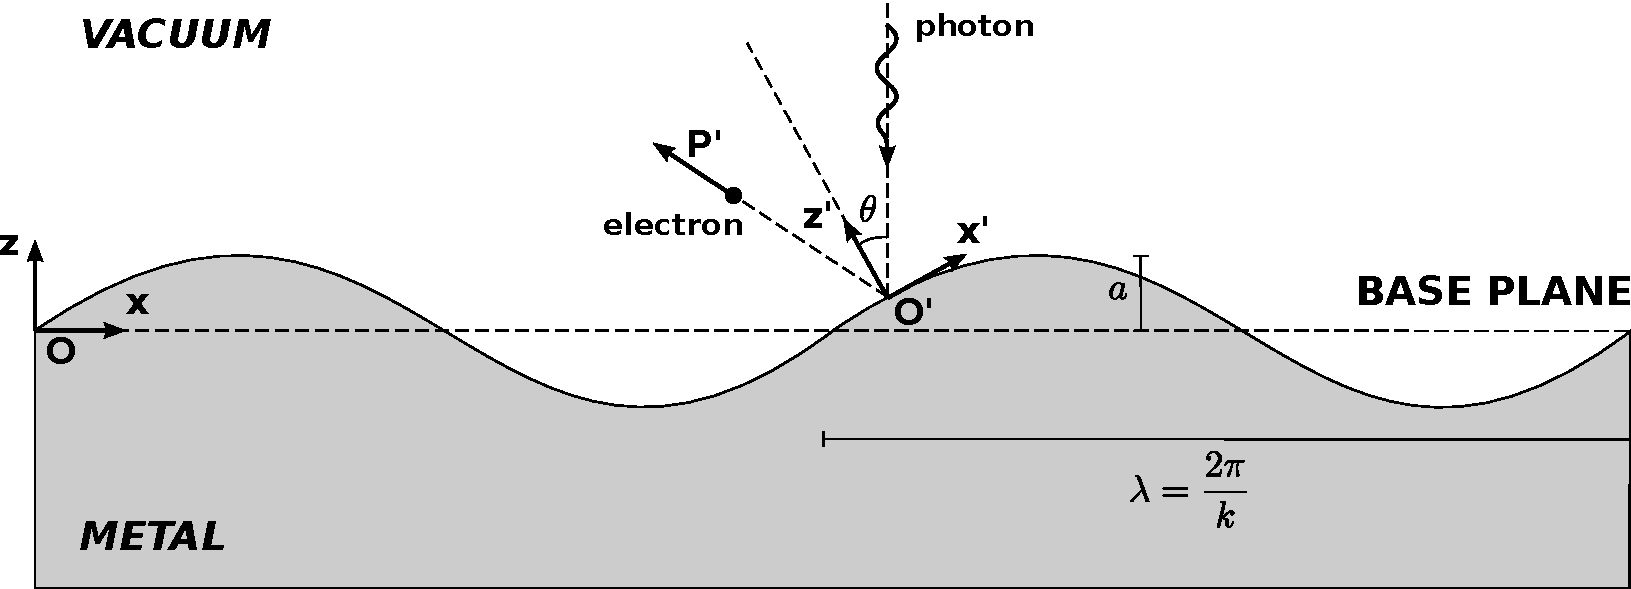
\includegraphics[width=0.9\textwidth]{coor_2D}
\caption{\label{fig:coor_2D} 2D 正弦表面的体发射示意图。坐标系统和参数的定义见图中标注。}
\end{figure}

如在节 \ref{ss:gmpsf} 中解释的那样,考虑在点 \textbf{P} 的入射,假设在全局坐标系下一个从点 \textbf{P} 发射出来的电子的横向和纵向动量分别为 $p_x, p_z$,应用 2D 旋转矩阵,我们有:
\[
\left(\begin{array}{c}
p_x\\
p_z
\end{array}\right)=
\left(\begin{array}{cc}
\cos\theta & -\sin\theta\\
\sin\theta & \cos\theta 
\end{array}\right)
\left(\begin{array}{c}
p_x^{\prime}\\
p_z^{\prime}
\end{array}\right)
\]
角度 $\theta$ 是从 z 轴到点 \textbf{P} 法向的夹角,且 $p_x^{\prime}, p_z^{\prime}$ 分别是发射电子在局部坐标系下的横向和纵向动量。上面的方程描述了发射角分散效应是如何影响横向动量,进而导致热发射度增长的。

现在考虑横向电场对发射度造成的影响。首先需要知道表面上横向电场的分布。有如下结论:定义 $\xi=ak$,那么若 $\xi$ 远小于 1,则正弦表面附近的电场可以写成下面形式:
\begin{eqnarray*}
E_x &=& E\xi\cdot e^{-kz}\sin kx \\
E_z &=& E\left(1+\xi e^{-kz}\cos kx\right)
\end{eqnarray*}
令 $A = eE/m$,可以证明,电子的横向动量近似满足下面的方程:
\[
p_{\infty}-p_0 = m\sqrt{\dfrac{\pi A}{2k}}\xi\sin kx
\]
其中 $p_{\infty}$ 是经历了阴极表面场后电子的最终横向动量。注意这里的横向动量应从极限的角度理解,即假定电子向 z 运动无穷远后,表面场对其横向的积分作用。事实上,电子的横向动量在离开表面几微米后就非常接近极限了。

将表面离散效应和横向电场效应叠加起来,就可以获得最终的 $p_x$ 的表达式:
\[
p_x = p_x^{\prime}\cos\theta-p_z^{\prime}\sin\theta + m\sqrt{\dfrac{\pi A}{2k}}\xi\sin kx
\]
其中:
\begin{eqnarray*}
\cos\theta &=&\dfrac{1}{\sqrt{1+\xi^2\sin^2kx}} \approx 1-\dfrac{1}{2}\xi^2\sin^2kx \\
\sin\theta &=&\dfrac{-\xi\sin kx}{\sqrt{1+\xi^2\sin^2kx}} \approx -\xi\sin kx
\end{eqnarray*}

将上面结果代入式 \ref{eq:emit_def},令 $p_C = m\sqrt{\pi A/2k}$($p_C$ 有动量的量纲),就得到式 \ref{eq:emit_2d} 所示的最终粗糙度发射度。这里我们定义式 \ref{eq:emit_2d} 中的方括号中的项的平方根为发射度增长因子 $\eta$,于是式 \ref{eq:emit_2d} 可以被重写为 $\varepsilon_x=\eta\cdot\varepsilon_{D, x}$。
\begin{equation}
\varepsilon_x^2 = \varepsilon_{D, x}^2\left[1+\dfrac{1}{2}\xi^2\left(\dfrac{\aver{\left(p_z^{\prime}+p_C\right)^2}}{\aver{{p_x^{\prime}}^2}}-1\right)\right]
\label{eq:emit_2d}
\end{equation}

当外场强度为 0 时,公式 \ref{eq:emit_2d} 就退化为表面离散效应粗糙度热发射度公式 \ref{eq:emit_2d_d};当 $p_z^{\prime} \ll p_C$ 时,式中的 $p_z^{\prime}$ 项可以忽略,从而公式 \ref{eq:emit_2d} 退化为横向电场效应粗糙度热发射度公式 \ref{eq:emit_2d_a}。
\begin{eqnarray}
\varepsilon_x^2 &\approx& \varepsilon_{D, x}^2\left(1+\frac{1}{2}\xi^2\right)\label{eq:emit_2d_d}\\
\varepsilon_x^2 &\approx& \varepsilon_{D, x}^2\left(1+\frac{3\pi e}{4}\cdot\frac{a^2kE}{\hbar\omega-\phi_{\text{eff}}}\right)\label{eq:emit_2d_a}
\end{eqnarray}

在式 \ref{eq:emit_2d} -- \ref{eq:emit_2d_a} 中代入表 \ref{tab:rough} 中的典型微观和宏观粗糙度参数,就可以看出对于微观粗糙度而言,发射度增长因子为 1.08,但是对于宏观粗糙度,发射度增长因子高达 1.35,这就意味着发射度增长主要是由宏观粗糙度导致的。分别保持 $\xi$ 和 $a$ 不变,画出粗糙度的空间周期 $\lambda$ 和发射度增长因子 $\eta$ 的关系,就得到图 \ref{fig:comp}。

\begin{figure}[htbp]
\centering
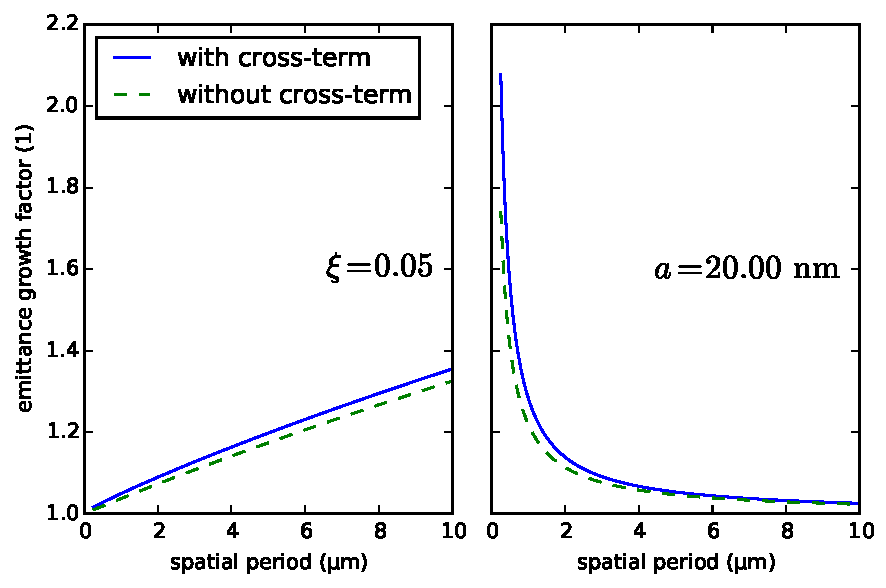
\includegraphics[width=0.7\textwidth]{comp}
\caption{\label{fig:comp} 2D 正弦表面上发射度增长因子与空间周期的关系。表面场强为 50\,MV/m。 左图是保持表面纹理的比例不变(即梯度不变,$\xi=0.05$);右图为保持表面振幅不变($a=20.00\,\text{nm}$)。}
\end{figure}

正如图 \ref{fig:comp} 中左图的实线所示,当等比例放缩表面纹理时,发射度增长因子和表面粗糙度空间周期是正相关的,这也验证了发射度增长的主要贡献来自宏观粗糙度的结论。我们也在图 \ref{fig:comp} 中检验了计算粗糙度热发射度时忽略表面离散效应和横向电场效应之间的耦合所造成的偏差,如图中虚线所示。容易看出实线和虚线间在某些空间周期时有着可观的差距,进一步的计算结果表明忽略两种效应耦合所造成的发射度增长的相对误差可达 10\%,这表明计算粗糙度热发射度时直接忽略两种效应的耦合有时是不合适的。

图 \ref{fig:comp} 说明了两个规律:1)阴极表面起伏越小,粗糙度热发射度增长越小;2)当阴极表面形状不变时,尺度越大,发射度增长就越大。图 \ref{fig:contour} 给出了一个关于空间周期,粗糙度振幅和发射度增长因子之间的更完整的理解。

\begin{figure}[htbp]
\centering
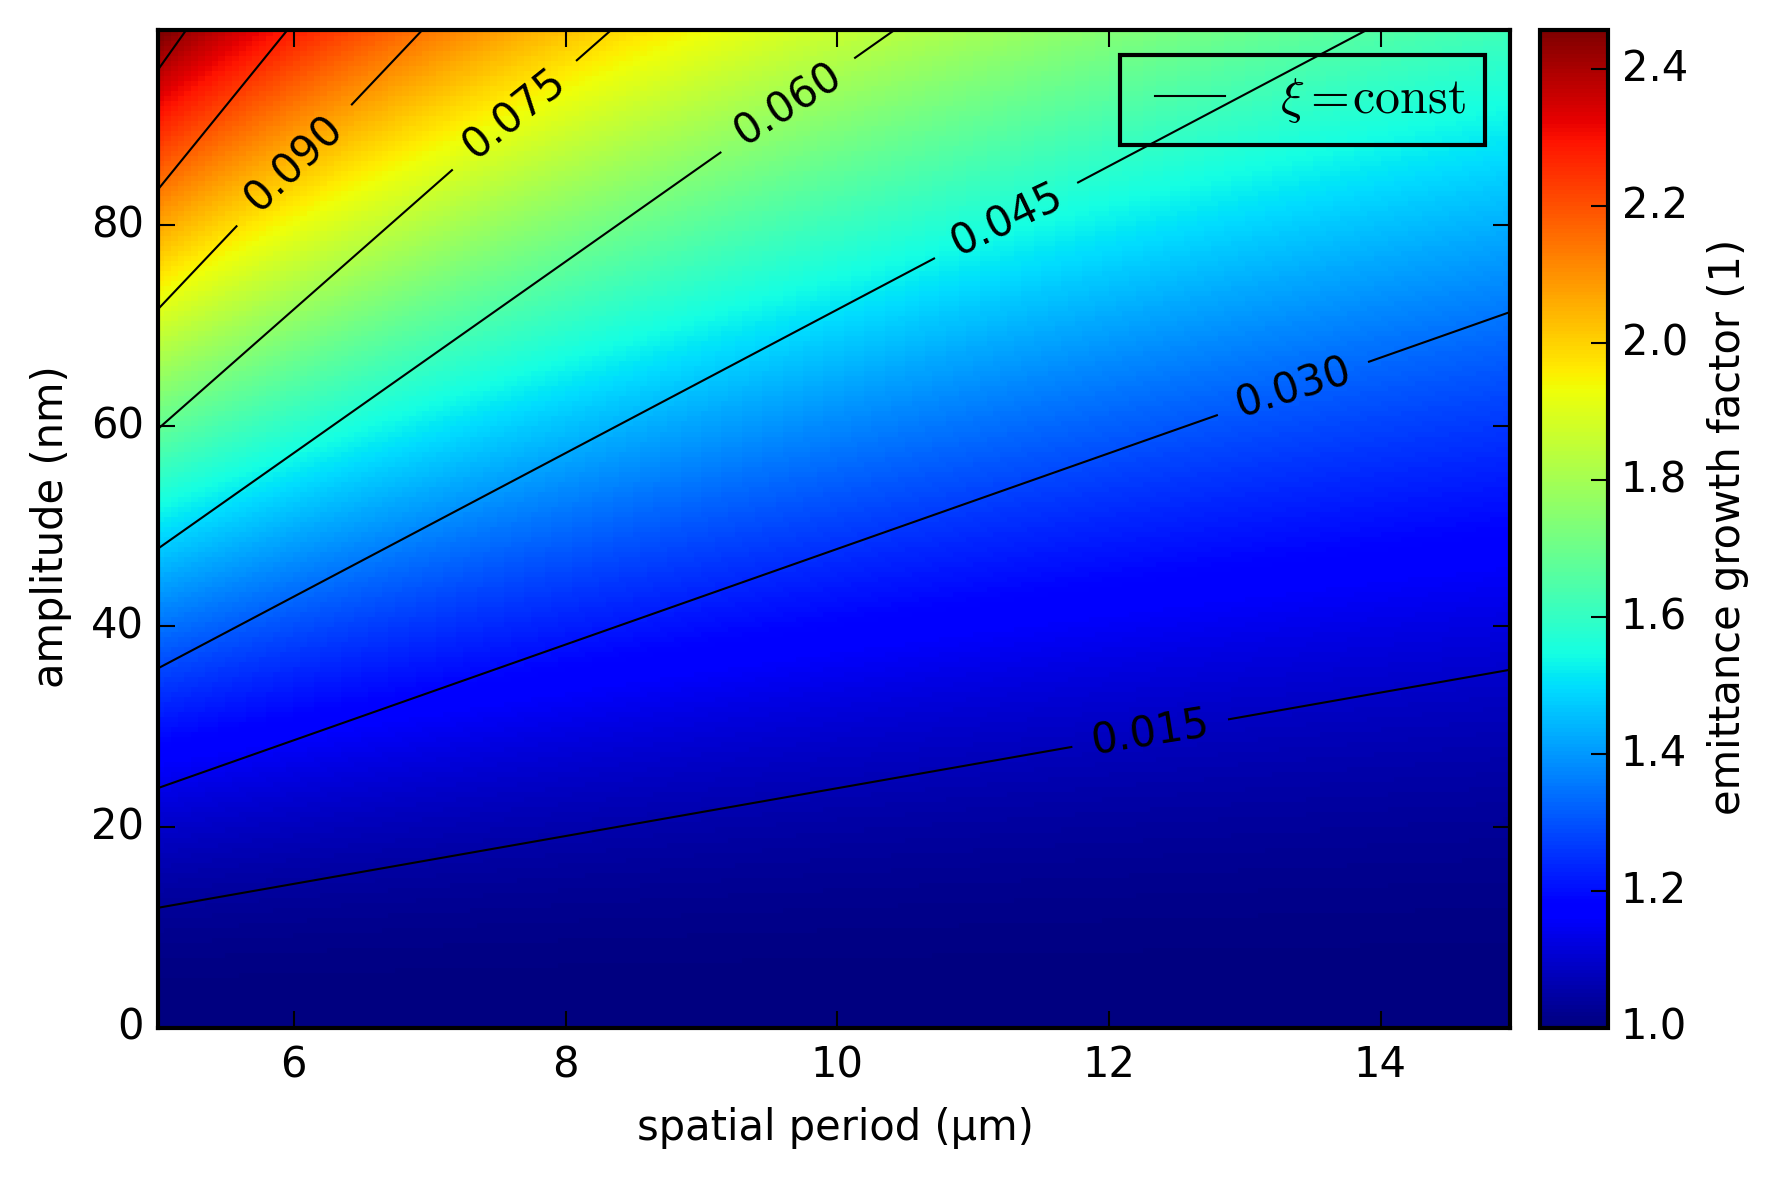
\includegraphics[width=0.6\textwidth]{contour}
\caption{\label{fig:contour} 发射度增长因子与表面粗糙度空间周期和振幅的关系。注意图中的黑色实线是表面形状(相同的形状 $\xi$ 相等)的等位线,而不是发射度增长因子的等位线,发射度增长因子相同则在图中颜色相同。}
\end{figure}

\subsection{\label{ss:2dr}2D 随机缓变粗糙表面}
现在我们研究 2D 随机缓变粗糙表面的情形,坐标系统如图 \ref{fig:coor_2Dr} 所示。
\begin{figure}[htbp]
\centering
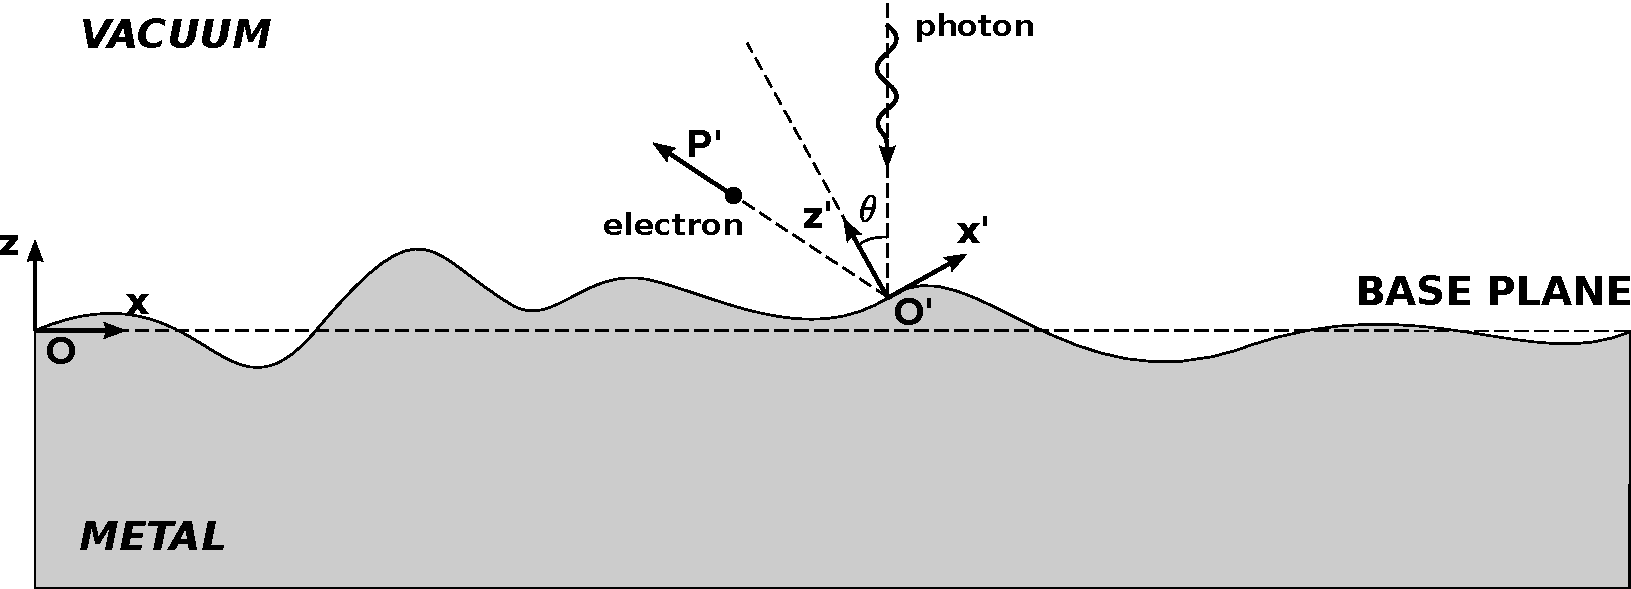
\includegraphics[width=0.9\textwidth]{coor_2Dr}
\caption{\label{fig:coor_2Dr} 2D 随机缓变粗糙表面的体发射示意图。坐标系统和参数的定义见图中标注。}
\end{figure}\\
计算 2D 随机缓变粗糙表面的粗糙度热发射度的思路与节 \ref{ss:2d} 中相同。表面离散效应造成的动量增长计算与节  \ref{ss:2d} 中的完全一致,所以我们跳过该部分而直接考虑横向电场效应部分。

假设表面形态函数为:
\[
z = R(x)
\]
我们选取基平面使得 $\langle R(x)\rangle=0$。和之前一样,想要计算横向场导致的横向动量增长,我们需要获取阴极表面附近的横向场分布。

\subsubsection{2D 随机缓变粗糙表面附近的电场分布}
受到 2D 正弦表面场分布计算的启发,我们可以假定在光阴极表面 $z = R(x)$ 与无穷远 $z = +\infty$ 之间的电势满足下面的近似形式:
\[
\phi(x, z) = z + \int dkC(k)\cdot e^{jkx-|k|z}
\]
上面的形式自动满足拉普拉斯方程 $\Delta\phi = 0$ 和 $z=\infty$ 处的边界条件 $\phi|_{z=d}=d, d\to\infty$,这里我们采用了归一化电场强度。现在考虑光阴极表面 $z=R(x)$ 处的边界条件。电势 $\phi$ 必须满足:
\[
\phi(x, z)\big|_{z=R(x)} = R(x) + \int dkC(k)\cdot e^{jkx-|k|R(x)} \equiv 0
\]
由于该表面为式 \ref{eq:def_gus} 所定义的随机缓变粗糙表面,$|k|R(x)$ 应该是一阶小量。将 $e^{-|k|R(x)}$ 做泰勒展开并保留一阶项就成为 $1-|k|R(x)$,代入上面的边界条件,就有:
\[
R(x) + \int dkC(k)\cdot e^{jkx} = O(1) \approx 0
\]
对 $R(x)$ 进行傅里叶展开:
\[
R(x) = \int dkR(k)\cdot e^{jkx}
\]
比较 $R(x)$ 的两个表达式,容易看出 $C(k) = -R(k)$,因此我们有二维随机缓变粗糙表面附近的电势 $\phi$ 的一阶近似表达式:
\begin{equation}
\label{eq:2d-pot}
\phi(x, z) = z - \int dkR(k)\cdot e^{jkx-|k|z}
\end{equation}

\begin{figure*}[htbp]
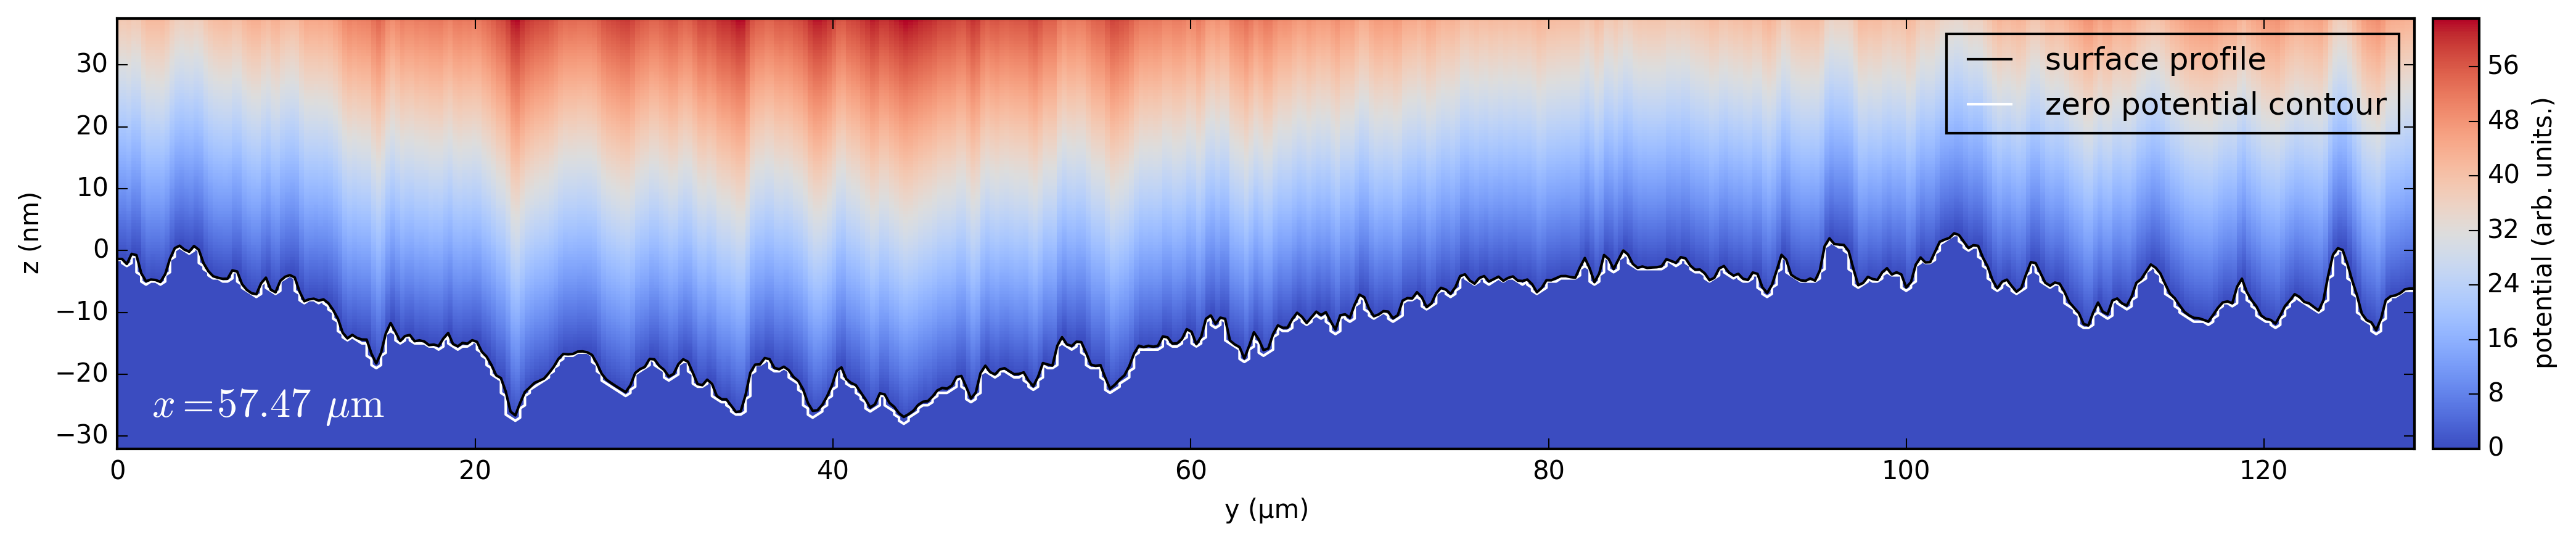
\includegraphics[width=\textwidth]{potential}
\caption{\label{fig:potential} 
验证电势一阶近似表达式的精确度。采用图 \ref{fig:conf} 所示的真实光阴极表面的沿 $x=57.47\,\mu\text{m}$ 的一个纵截面,该截面阴极表面轮廓用黑色实现描出;图中的白色实线为式 \ref{eq:2d-pot} 给出的解析公式的零势能面(对于 2D 情形而言是一条曲线),从图中可见看到,阴极表面轮廓和解析的零势能面几乎完全重合,这就验证了电势一阶近似表达式的精确性。}
\end{figure*}

为了验证上面的近似公式,我们选择了一个二维随机缓变粗糙表面,同时画出表面轮廓和近似的电势图。由于推导中我们假设阴极表面电势为 0,因此近似公式中的零势能面就描绘了解析的表面轮廓。实际的表面轮廓与解析的表面轮廓越接近,该一阶近似公式就越精确。二者的比较见图 \ref{fig:potential}。

从图 \ref{fig:potential} 中可以看到,二维随机缓变粗糙表面附近的电势一阶近似表达式是足够精确的。利用电势和电场间的关联 $\bm{E}=-\nabla\phi$,就可以得到表面附近的近似电场分布:
\begin{eqnarray*}
E_x &=& j\int dk\cdot kR(k)\cdot e^{jkx-|k|z} \\
E_z &=& -1-\int dk\cdot |k|R(k)\cdot e^{jkx-|k|z}
\end{eqnarray*}

\subsubsection{2D 随机缓变粗糙表面的粗糙度热发射度}

现在假定表面场强为 $E$,由牛顿第二定律可以写出:
\begin{eqnarray}
p_{\infty}-p_0 &=& m\sqrt{\dfrac{A}{2}}\cdot\int-\dfrac{E_x}{\sqrt{z}}\,dz\nonumber\\
&=& -jm\sqrt{\dfrac{\pi A}{2}}\cdot\int dk \dfrac{k}{\sqrt{|k|}}R(k)\cdot e^{jkx}\label{eq:p_field}
\end{eqnarray}
代入统计意义发射度公式计算可得最终发射度为:
\begin{equation}
\varepsilon_x^2 = \varepsilon_{D, x}^2\left[1-\aver{{R^{\prime}}^2}+\dfrac{\aver{\left(p_z^{\prime}\cdot R^{\prime}+jm\sqrt{\dfrac{\pi A}{2}}\displaystyle\cdot\int dk \dfrac{k}{\sqrt{|k|}}R(k)\cdot e^{jkx}\right)^2}}{\aver{{p_x^{\prime}}^2}}\right]
\label{eq:emit_2dr}
\end{equation}

为验证式 \ref{eq:emit_2dr} 的正确性,我们考虑节 \ref{ss:2d} 中所考虑的特殊二维情形,即二维正弦表面 $R(x) = a\cos k_0x$,为推导方便这里假定 $k_0>0$。令:
\[
I(x) = jm\sqrt{\dfrac{\pi A}{2}}\displaystyle\cdot\int dk \dfrac{k}{\sqrt{|k|}}R(k)\cdot e^{jkx}
\]
而 $R(k)=\frac{a}{2}\left[\delta(k-k_0)+\delta(k+k_0)\right]$,因此:
\begin{eqnarray*}
I(x) &&= jm\sqrt{\dfrac{\pi A}{2}}\left[\frac{a}{2}\dfrac{k_0}{\sqrt{|k_0|}}e^{jk_0x}-\frac{a}{2}\dfrac{k_0}{\sqrt{|k_0|}}e^{-jk_0x}\right]\\
&&= m\sqrt{\dfrac{\pi A}{2k_0}}\cdot(-ak_0\sin k_0x) = p_C\cdot R^{\prime}
\end{eqnarray*}
从而:
\begin{eqnarray*}
\varepsilon_x^2 &&= \varepsilon_{D, x}^2\left[1-\aver{{R^{\prime}}^2}+\dfrac{\aver{\left(p_z^{\prime}\cdot R^{\prime}+I(x)\right)^2}}{\aver{{p_x^{\prime}}^2}}\right]\\
&&= \varepsilon_{D, x}^2\left[1+\aver{{R^{\prime}}^2}\left(\dfrac{\aver{\left(p_z^{\prime}+p_C\right)^2}}{\aver{{p_x^{\prime}}^2}}-1\right)\right]\\
&&= \varepsilon_{D, x}^2\left[1+\dfrac{1}{2}\xi^2\left(\dfrac{\aver{\left(p_z^{\prime}+p_C\right)^2}}{\aver{{p_x^{\prime}}^2}}-1\right)\right]
\end{eqnarray*}
结果与式 \ref{eq:emit_2d} 相同。这就意味着对于二维缓变正弦表面,公式 \ref{eq:emit_2dr} 退化为公式 \ref{eq:emit_2d},这样我们就验证了二维随机缓变粗糙表面粗糙度热发射度公式 \ref{eq:emit_2dr} 的可靠性。

另外,$I(x)$ 也可以被写成下面的等价形式:
\begin{equation}
I(x) = \frac{m}{2}\sqrt{\frac{A}{|x|}}\ast R^{\prime}(x)
\label{eq:conv}
\end{equation}
利用卷积定理以及下面恒等式:
\[
\mathcal{F}\left(\dfrac{1}{\sqrt{|x|}}\right) = \frac{\sqrt{2\pi}}{|k|}
\]
其中 $\mathcal{F}\left(f(x)\right) = \int f(x)e^{-jkx}dx$ 是 $f(x)$ 的傅里叶变换,我们就可以直接得到式 \ref{eq:emit_2d} 的结果。

\subsection{\label{ss:3d}3D 随机缓变粗糙表面}
采用和节 \ref{ss:2dr} 相似的思想,可以解决三维随机缓变粗糙表面上粗糙度热发射度计算的问题。假定三维随机缓变粗糙表面可用下式描述:
\[
z = R(x, y)
\]
依然选取基平面使得 $\langle R(x, y)\rangle=0$。

\subsubsection{3D 随机缓变粗糙表面附近的电场分布}
仿照二维情形,我们假定光阴极表面 $z = R(x, y)$ 和无穷远 $z = +\infty$ 之间的电势有下面的近似形式:
\[
\phi(x, y, z) = z + \int dk_xdk_yC(k_x, k_y)\cdot e^{j(k_xx+k_yy)-kz}
\]
其中 $k=\sqrt{k_x^2+k_y^2}$。容易证明上面的形式自动满足拉普拉斯方程和无穷远处边界条件。结合阴极表面的边界条件,我们有 $C(k_x, k_y)=-R(k_x, k_y)$,其中 $R(k_x, k_y)$ 是 $R(x, y)$ 的傅里叶变换系数。于是电势可写成:
\[
\phi(x, y, z) = z - \int dk_xdk_yR(k_x, k_y)\cdot e^{j(k_xx+k_yy)-kz}
\]
进而电场具有以下形式:
\begin{eqnarray*}
E_x &=& j\int dk_xdk_y\cdot k_xR(k_x, k_y)\cdot e^{j(k_xx+k_yy)-kz} \\
E_y &=& j\int dk_xdk_y\cdot k_yR(k_x, k_y)\cdot e^{j(k_xx+k_yy)-kz} \\
E_z &=& -1-\int dk_xdk_y\cdot kR(k_x, k_y)\cdot e^{j(k_xx+k_yy)-kz}
\end{eqnarray*}

\subsubsection{3D 随机缓变粗糙表面的粗糙度热发射度}
现在考虑发射光电子的横向动力学,有:
\begin{eqnarray}
p_{\infty}-p_0 &=& m\sqrt{\dfrac{A}{2}}\cdot\int-\dfrac{E_x}{\sqrt{z}}\,dz\\\label{eq:p_field_3d}
&=& -jm\sqrt{\dfrac{\pi A}{2}}\cdot\int dk_xdk_y\dfrac{k_x}{\sqrt{k}}R(k_x, k_y)\cdot e^{j(k_xx+k_yy)}\nonumber
\end{eqnarray}

类似节 \ref{ss:2dr},不难推出三维随机缓变粗糙表面光阴极的粗糙度热发射度如式 \ref{eq:emit_3d} 所示。

\begin{equation}
\varepsilon_x^2 = \varepsilon_{D, x}^2\left[1-\aver{\partial_x^2R}+\dfrac{\aver{\left(p_z^{\prime}\cdot\partial_xR+jm\sqrt{\dfrac{\pi A}{2}}\displaystyle\cdot\int dk_xdk_y\dfrac{k_x}{\sqrt{k}}R(k_x, k_y)\cdot e^{j(k_xx+k_yy)}\right)^2}}{\aver{{p_x^{\prime}}^2}}\right]
\label{eq:emit_3d}
\end{equation}

和 2D 情形类似,将 $E = 0$ 代入式 \ref{eq:emit_3d},就可以得到三维表面离散效应粗糙度热发射度式 \ref{eq:emit_3d_d}。
\begin{equation}
\varepsilon_x^2 = \varepsilon_{D, x}^2\Big(1+\aver{\partial_x^2R}\Big)
\label{eq:emit_3d_d}
\end{equation}
由傅里叶能量守恒定律,$\aver{\partial_x^2R}$ 项可以被写成下面的等价形式:
\[
\left\langle \partial_x^2 R \right\rangle = \dfrac{\displaystyle\iint_{F(S)} k_x^2\left|R(k_x, k_y)\right|^2dk_xdk_y}{\displaystyle\iint_{S} dxdy}
\]
注意到空间谐波振幅 $|R(k_x, k_y)|$ 和空间谐波波数 $k_x$ 的乘积即为形状参数 $\xi$,而在 2D 正弦表面情形中,$\xi$ 参数正比于表面离散效应对粗糙度热发射度的贡献,因此这个对 2D 正弦表面成立的结论对于一般的随机缓变三维表面也成立,这同时意味着 2D 和 3D 的结果是自洽的。

尽管 3D 随机表面粗糙度热发射度形式上比 2D 正弦表面的要复杂,我们依然可以从公式 \ref{eq:emit_3d} 中得到一些有用的规律。例如,我们考虑发射度增长因子 $\eta$ 随外加电场强度 $E$ 的关系,将式 \ref{eq:emit_3d} 对 $E$ 展开就有:
\[
\eta^2 = aE+b\sqrt{E}+c
\]
这里 $a, b$ 和 $c$ 是只与阴极表面形状相关的参数。一些实验结果已经验证了 $E$ 和 $\varepsilon$ 具有类似的二次关系。

\section{\label{s:num}数值模拟验证}
\subsection{光阴极的量子效率与表面形态的关系}
在节 \ref{ss:gmpsf} 中,计算发射度时我们忽略了相对量子效率(或发射权重) $W(\theta)$ 与该点入射光子与表面法向之间夹角 $\theta$ 之间的关联,现在详细研究这二者之间的关系。铜光阴极的反射率 $R(\theta)$ 与发射权重 $W(\theta)$ 与入射角 $\theta$ 之间的关系如图 \ref{fig:weight} 中所示。
\begin{figure}[htbp]
\centering
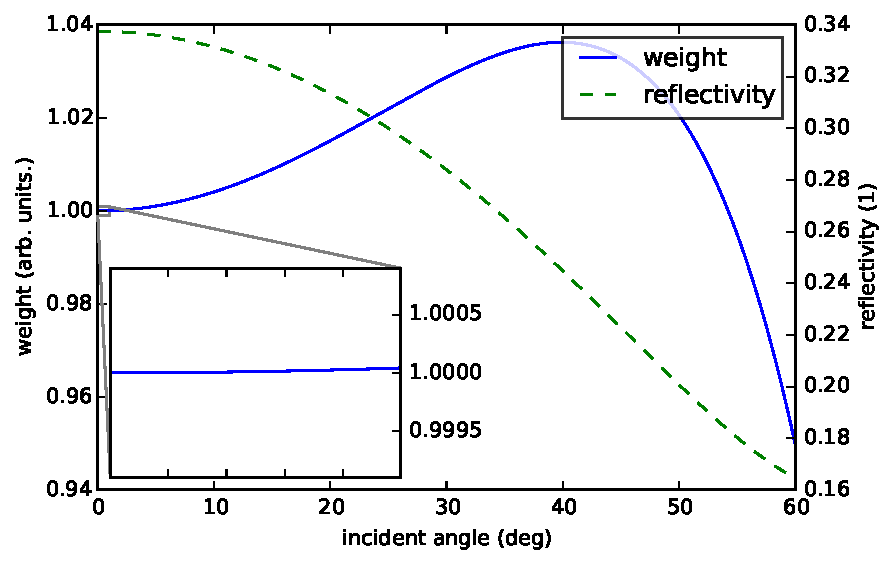
\includegraphics[width=0.6\textwidth]{weight}
\caption{\label{fig:weight} 相对量子效率 $W(\theta)$ 与反射率 $R(\theta)$ 与入射角 $\theta$ 之间的关系。相对量子效率 $W(\theta)$ 正比于阴极上该点处的光电子发射密度。图中图放大了 0 度到 1 度之间的相对量子效率曲线。}
\end{figure}
图 \ref{fig:weight} 也展示了 0 度到 1 度之间的相对量子效率曲线。容易看出在 1 度以下,相对量子效率基本是常数。这就是在发射度计算中忽略 $W(\theta)$ 和 $\theta$ 之间关系的原因。在以下的数值模拟中,$W(\theta)$ 也会被做为常量处理。

\subsection{\label{ss:sim-conf}数值模拟配置}
整个数值模拟程序采用 Python 编写,其模拟的场景如图 \ref{fig:conf} 所示。图中央区域的蓝红渐变区域代表激光入射区域,背景取自一块真实光阴极的表面的白光干涉仪测量结果。这块表面的空间频谱如图 \ref{fig:spec} 所示。阴极材料是无氧铜(阴极材料会影响阴极的逸出功,电子和光子的平均自由程,进而影响量子效率和发射度)。为模拟横向电场效应,我们在该表面引入了一个高场强电场,简单起见,采用了恒定场代替射频场,由于激光的脉冲长度远小于电子枪中射频场的周期,这个近似也是符合实际的。
\begin{figure}[htbp]
\centering
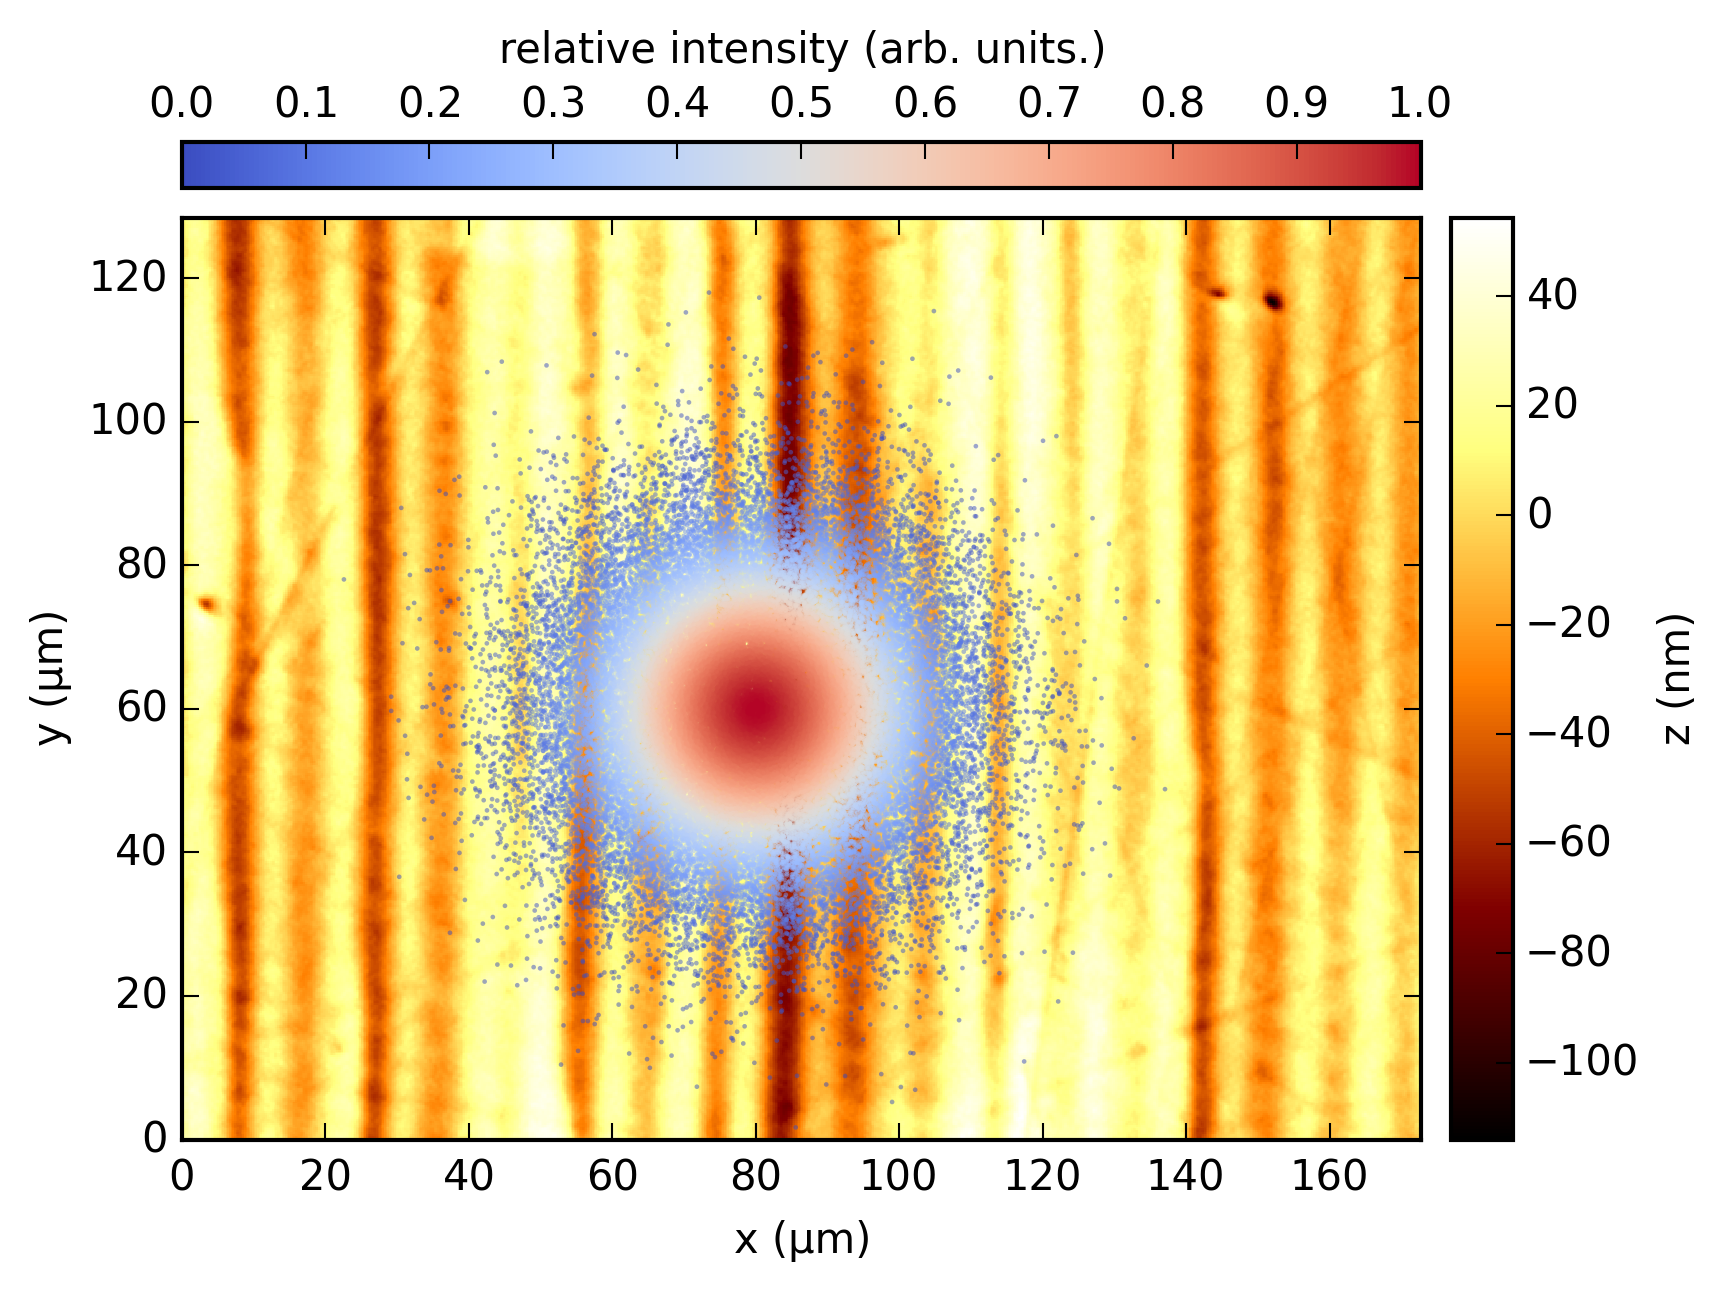
\includegraphics[width=0.6\textwidth]{configuration}
\caption{\label{fig:conf} 数值模拟配置。黄黑渐变的背景代表了模拟中所使用的表面的形态分布,中心附近红蓝渐变的区域描述了激光的横向功率密度分布。}
\end{figure}

\begin{figure}[htbp]
\centering
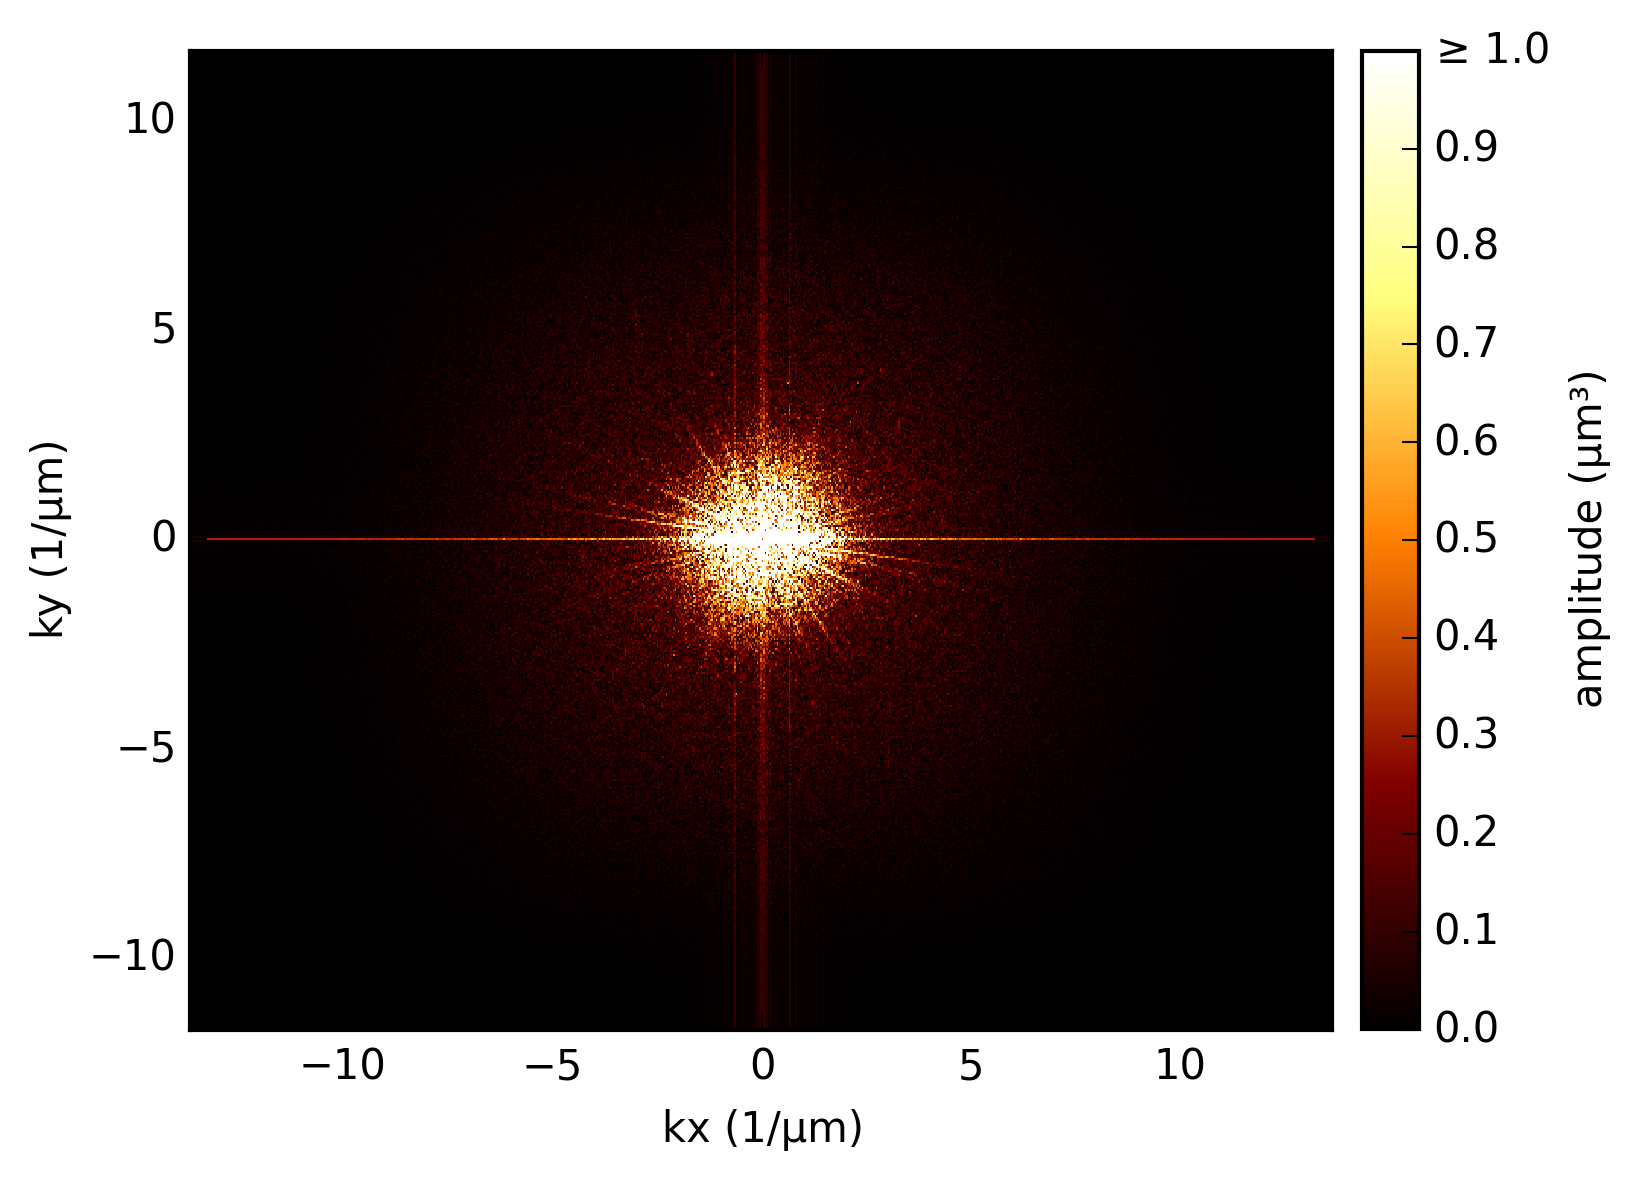
\includegraphics[width=0.6\textwidth]{spectrum}
\caption{\label{fig:spec} 模拟中采用的表面的空间频谱。为了使高频成分也可见,我们设置了饱和振幅为 1\,$\mu\text{m}^{3}$,也就是说变换后所有幅度大于 1\,$\mu\text{m}^{3}$ 的空间分量其振幅都当作 1\,$\mu\text{m}^{3}$ 来绘制。}
\end{figure}

在上面的配置下,我们对阴极表面的光电子进行动力学模拟,之后对初始发射度与饱和发射度进行统计,从而获得不同模拟参数下的发射度增长因子。

\subsection{\label{ss:sim-prin}数值模拟原理}
粗糙度热发射度可以分为两部分,即表面离散效应和横向电场效应导致的热发射度,进行数值模拟时需要对二者分别处理。总体而言,模拟需要一块特定材料的粗糙表面,一个外加场强与一束激光。我们采用了一块真实铜阴极的表面形态数据(白光干涉仪测量得到)做为特定材料的粗糙表面,其光学参数可以查阅得到;为了生成阴极表面上的外加电场,应用了节 \ref{ss:3d} 中给出的电场分布公式;为获得被给定横向功率密度分布的激光照射而出射的初始电子束团,首先生成符合激光横向功率密度分布的二维位置序列,随后对每个位置赋予一个概率分布为该点动量点扩散函数(由于法向不同,表面各点的动量点扩散函数有微小差异)的随机动量,最后将位置序列与随机动量合并,就得到了符合初始电子束相空间的一组采样。

有了初始电子束团,需要对其进行动力学模拟以给出发射度演变过程,这可以应用 5 阶龙格库塔法对运动方程进行积分。出于统计的方便,我们采用了以纵向位置坐标 $z$ 做为积分变量的方式,而不是以时间 $t$ 做为积分变量。以 $z$ 为变量的电子运动方程为:
\begin{eqnarray*}
\frac{dp_x\,[\text{keV/c}]}{dz\,[\text{nm}]} &=& 511\times 10^{-6}\cdot\frac{E_0\,[\text{MV/m}]}{p_z\,[\text{keV/c}]}\cdot \hat{E}_x(x, y, z)\\
\frac{dx\,[\mu\text{m}]}{dz\,[\text{nm}]} &=& \frac{p_x\,[\text{keV/c}]}{p_z\,[\text{keV/c}]}\cdot 1\times 10^{-3}
\end{eqnarray*}
其中 $x$ 代表横向,$E_0$ 是阴极表面电场强度,$\hat{E}_x$ 是归一化横向电场分布。值得注意的是,考虑到缓变表面的特征与模拟的目的,我们选取了 $\mu$m 做为横向尺寸的单位,nm 做为纵向尺寸单位。

从阴极表面电场分布的公式上可看出,电场的横向分量随着到基平面距离的增大而指数衰减,因此光电子的横向动量一定会很快饱和。通过实际模拟发现,饱和距离可以选在距离基平面 5000\,nm 附近,我们就在饱和距离处进行发射度增长因子的统计。

\subsection{\label{ss:sim-res}数值模拟结果}
数值模拟参数参见表 \ref{tab:sim1},发射度演变结果见图 \ref{fig:sim1}。
\begin{table}[htbp]
\centering
\caption{\label{tab:sim1}
数值模拟中所用参数。}
\begin{tabular}{llll}
\toprule
参数 & 值 & 单位 & 描述\\
\midrule
$\lambda_l$ & 266.0 & nm & 激光波长 \\
l-dist & \text{均匀分布} & - & 激光横向分布 \\
$r_l$ & 20.0 & $\mu$m & 激光横向半径 \\
$x_l$ & 80.0 & $\mu$m & 激光入射中心横座标 \\
$y_l$ & 60.0 & $\mu$m & 激光入射中心纵座标 \\
mat & \text{无氧铜} & - & 光阴极材料 \\
$E_0$ & 50.0 & MV/m & 阴极表面有效电场强度 \\
$\phi_w$ & 4.31 & eV & 阴极逸出功 \\
$\phi_{\text{eff}}$ & 4.04 & eV & 阴极有效逸出功 \\
$E_F$ & 7.0 & eV & 材料费米能级 \\
$N$  & 10000 & - & 模拟所用粒子数 \\
$z_i$ & 0 & nm & 模拟起始位置 \\
$z_f$ & 5000.0 & nm & 模拟结束位置 \\
$dz$ & 10.0 & nm & 模拟步长 \\
\bottomrule
\end{tabular}
\end{table}

从图 \ref{fig:sim1} 中可看到,在运动过程中,束团相空间沿着 $x$ 方向逐渐扭曲。相空间扭曲的原因就是表面的横向电场,而正是相空间扭曲导致了发射度增长。分别对初始相空间和结束相空间进行统计,可以得到发射度增长因子:
\[
\eta_{s} = \frac{\varepsilon_f}{\varepsilon_i} = \frac{4.826\,\mu\text{m}\cdot\text{keV}/c}{4.623\,\mu\text{m}\cdot\text{keV}/c} = 1.044
\]
令人惊讶的是,发射度增长因子比大部分文献中报道的(1.5 $\sim$ 2)要小得多!我们的模拟结果说明了表面粗糙度效应可能并非实验中观测到的发射度增长的唯一原因。

\begin{figure}[htbp]
\centering
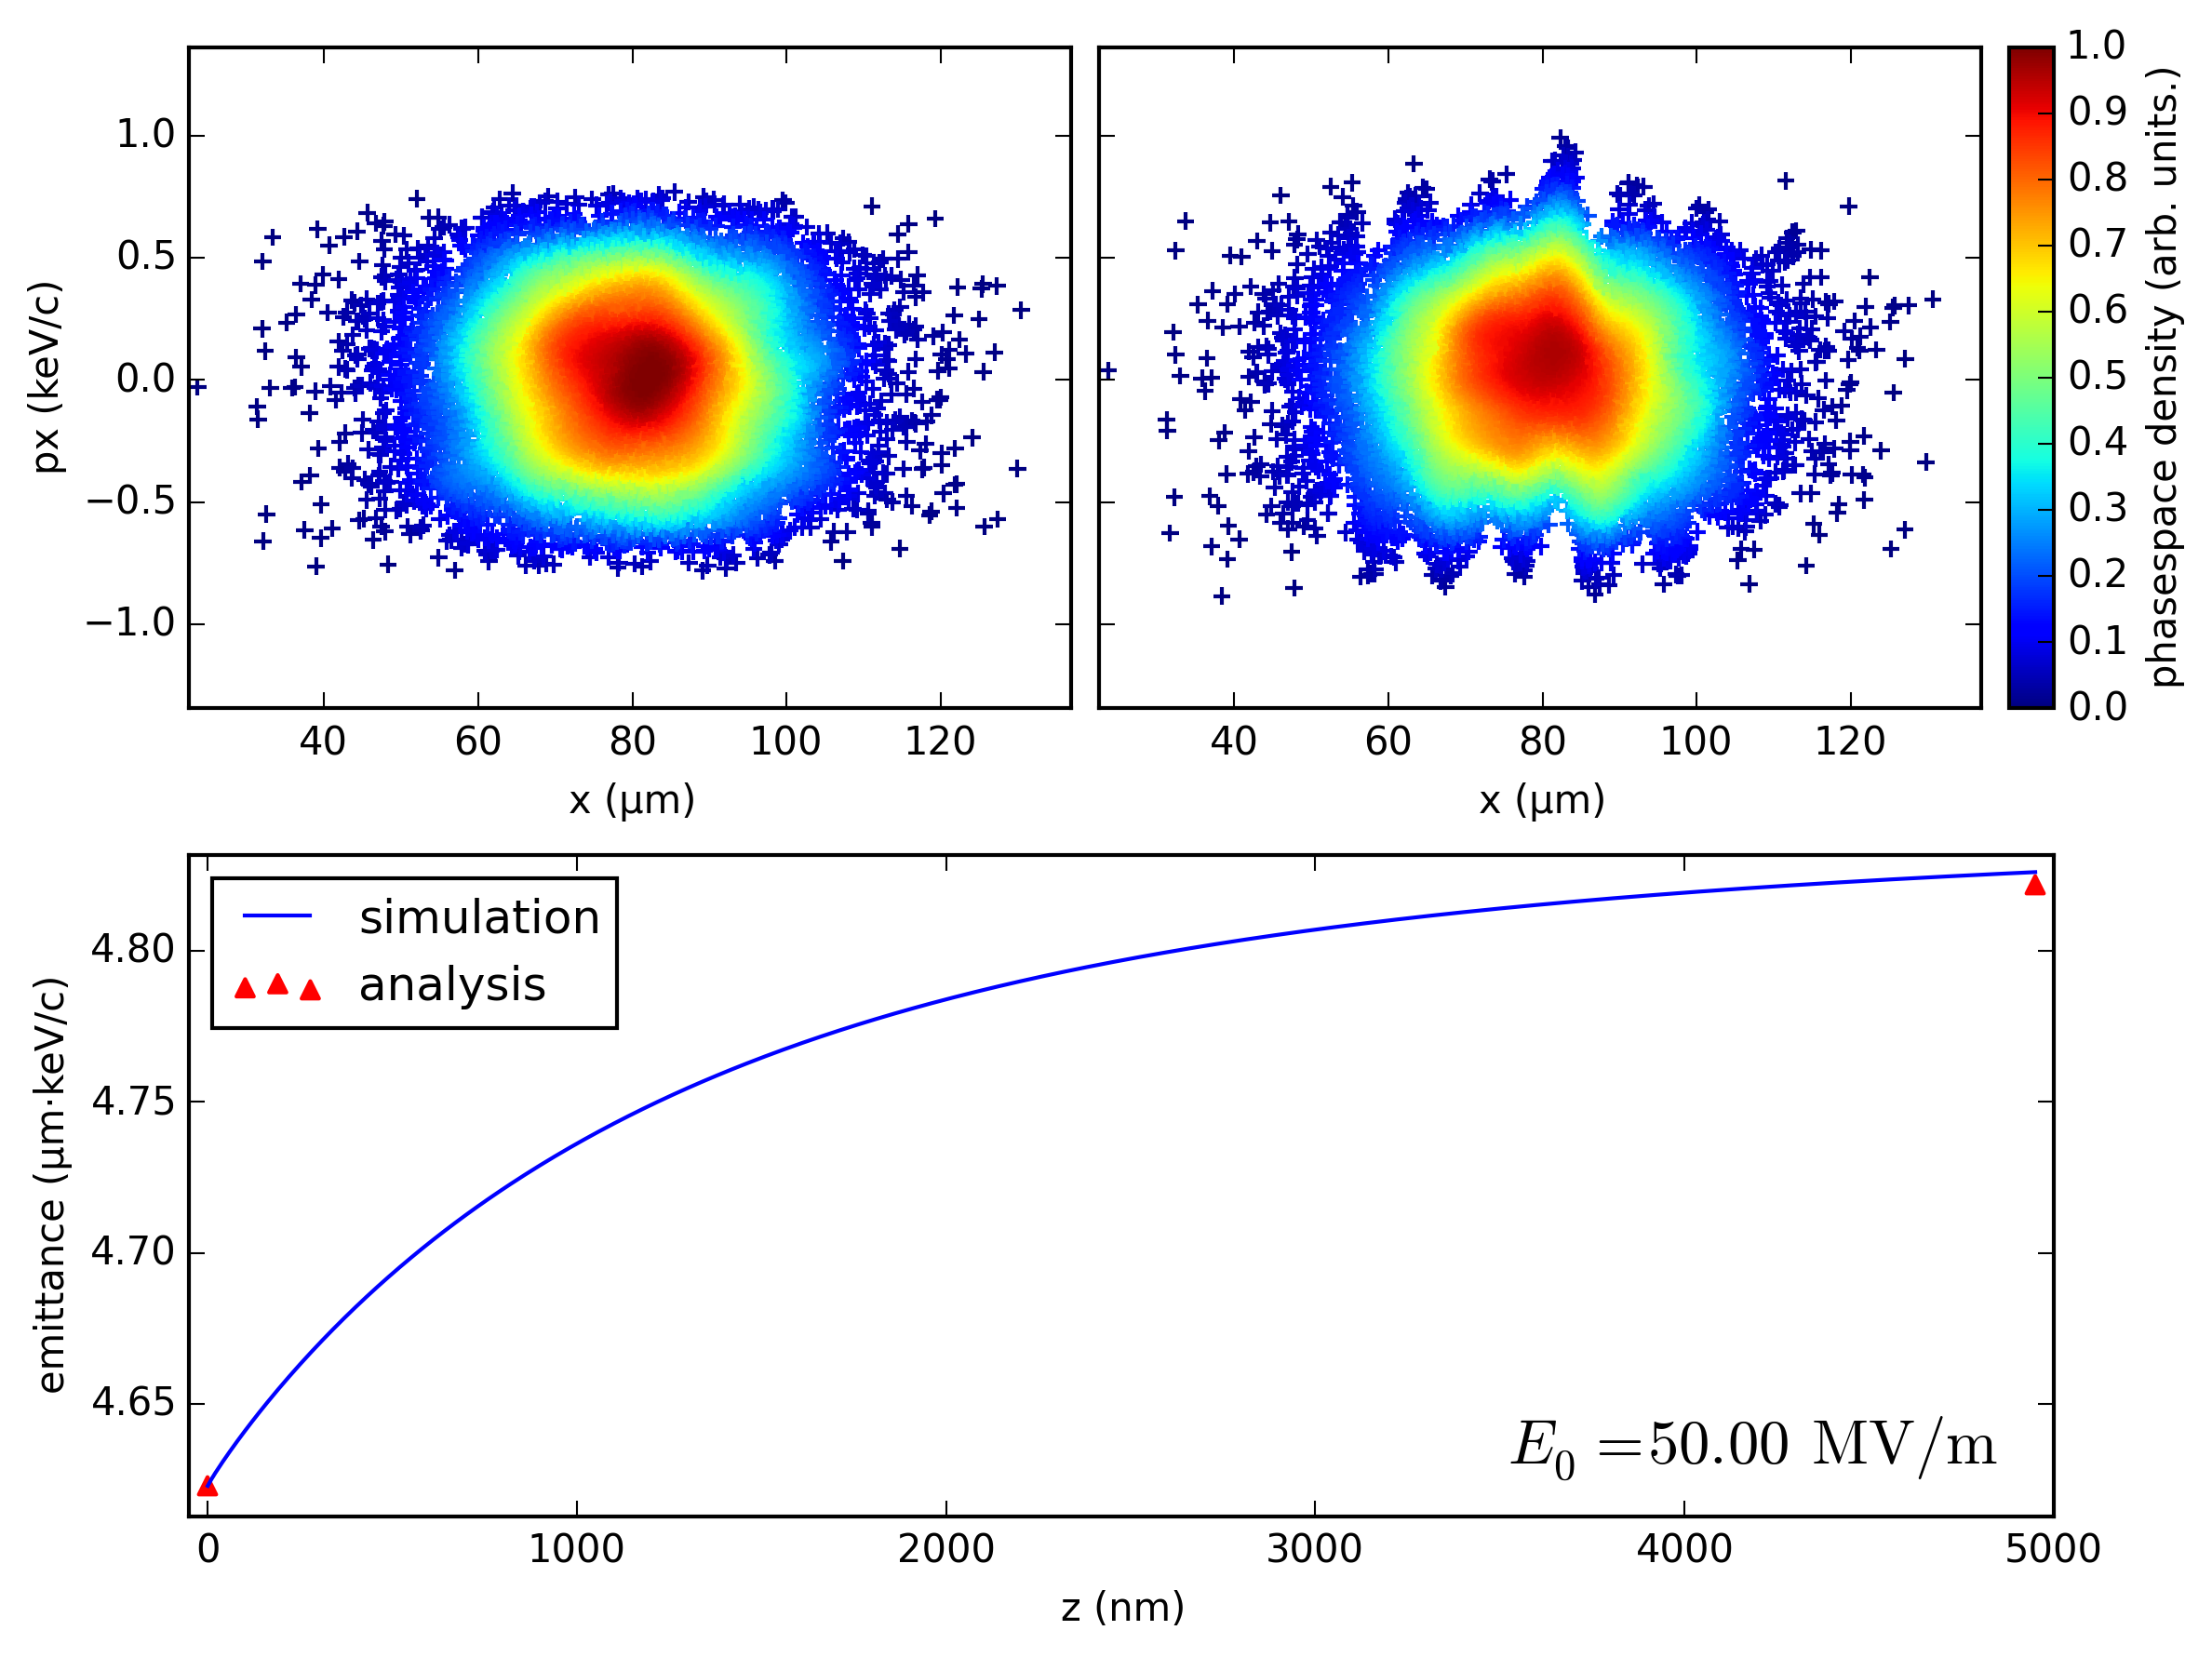
\includegraphics[width=0.6\textwidth]{simulation}
\caption{\label{fig:sim1} 
图 \ref{fig:conf} 中所示的粗糙铜阴极表面的电子束相空间与发射度演变的模拟结果。左上图是 $z=0\,\text{nm}$ 处的初始相空间分布,右上图是 $z=5000\,\text{nm}$ 处的最终相空间分布,下图是发射度 $\varepsilon_x$ 沿 $z$ 的演变,其中左右两个红色三角符号分别是解析初始发射度与解析饱和发射度。}
\end{figure}

\subsection{\label{ss:sim-res}数值模拟与解析结果的对比}
我们在图 \ref{fig:sim1} 中比较了粗糙度发射度的模拟结果与解析结果(见公式 \ref{eq:emit_3d})。图中的两个红色三角形符号代表解析结果:左边的是只考虑了表面离散效应的粗糙度热发射度,($\varepsilon_1$),右边则是将横向电场效应一起加入的粗糙度热发射度($\varepsilon_2$)。由于模拟中在产生初始电子束团时,已经包含了表面离散效应,而且采用了相同的电子束团进行理论计算和模拟模拟,因此 $\varepsilon_1$ 对于理论和模拟而言是完全相同的。

对于 $\varepsilon_2$,理论上说模拟结果应该比解析结果略小并且随着纵向位置 $z$ 的增大逐渐趋于解析结果,但是图 \ref{fig:sim1} 中却正相反。这可能是因为我们的模拟步长选得过大导致的,因为横向电场分布会随着 $z$ 的增大而衰减,所以运动方程积分会比真实的动量改变要大(因为龙格库塔法中每步所采用的外场都是上一时刻的场),进而导致模拟结果比解析结果略大。

尽管如此,解析公式给出的最终发射度增长因子为:
\[
\eta_a = \frac{\varepsilon_2}{\varepsilon_1} = \frac{4.822\,\mu\text{m}\cdot\text{keV}/c}{4.623\,\mu\text{m}\cdot\text{keV}/c} = 1.043
\]
可以看出解析结果与数值模拟结果相当接近,这就进一步验证了解析结果的可靠性。

应用粗糙度发射度的解析公式,发射度增长因子的计算速度可以大大提高,所以可以借助解析公式来探索阴极表面电场强度与发射度增长因子之间的关系。分析结果见图 \ref{fig:factor_comp} 中蓝色实线。图 \ref{fig:factor_comp} 说明,对于经过打磨的光阴极,其由于三维表面粗糙度造成的发射度增长是很小的,即使在阴极表面场高达 120\,MV/m 的情形下,发射度增长因子仍然小于 1.1。

\begin{figure}[htbp]
\centering
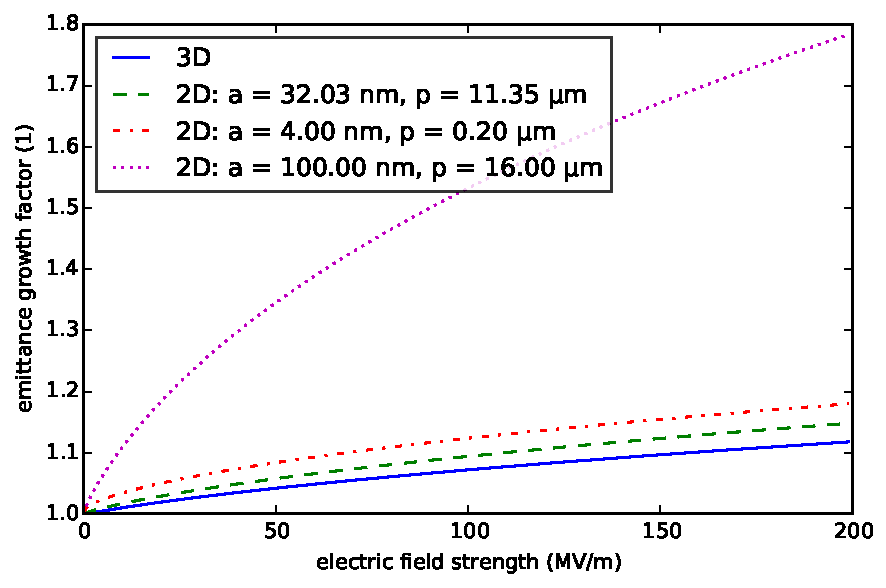
\includegraphics[width=0.6\textwidth]{factor_comp}
\caption{\label{fig:factor_comp} 2D 粗糙表面和 3D 粗糙表面的发射度增长因子对比。蓝色实线对应图 \ref{fig:conf} 中所示的粗糙阴极表面的发射度增长因子;绿色虚线代表粗糙度参数和 3D 粗糙表面相同的 2D 近似公式给出的增长因子;红色点划线和洋红色点虚线分别对应表 \ref{tab:rough} 中的微观粗糙度和宏观粗糙度参数对应的 2D 近似公式给出的增长因子。}
\end{figure}

图 \ref{fig:factor_comp} 中同时比较了若干粗糙度参数不同的 2D 正弦表面与 3D 随机缓变粗糙表面的发射度增长。对于 2D 正弦表面,我们采用了三组不同的粗糙度空间周期 $p$ 和粗糙度振幅 $a$,具体说明见图 \ref{fig:factor_comp} 题注。可以看出,在表面场强相同的情况下,2D 宏观粗糙度的发射度增长因子明显高于 3D 真实阴极表面的发射度增长因子。但是由于 3D 表面的粗糙度参数 $a$ 和 $p$ 与宏观粗糙度的参数有很大差异,这种比较并无太大意义。为了获得更有意义的比较结果,我们统计了图 \ref{fig:conf} 所示的粗糙表面的粗糙度参数,得到其 rms 粗糙度 $R_q$ 和 rms 平均空间波长 $\lambda_q$ 分别为 22.65\,nm 和 11.35\,$\mu$m。对应的 2D 正弦表面若想达到相同的粗糙度参数,其空间周期 $\lambda$ 和振幅 $a$ 需要满足下式:
\begin{eqnarray*}
&&a = \sqrt{2}R_q \\
&&\lambda = \lambda_q
\end{eqnarray*}
计算得到 $a=32.03\,\text{nm}$,$\lambda=11.35\,\mu\text{m}$。应用这组参数,画出对应的发射度增长因子曲线如图 \ref{fig:factor_comp} 中的绿色虚线所示。可以看出,对于拥有相同粗糙度参数的 3D 和 2D 表面,其发射度增长因子是非常接近的,但是 3D 情形总是比 2D 情形的发射度增长因子更小。这个现象的原因可能是 3D 表面的横向动量增长是分散在整个 x-y 平面的,但是 2D 表面的横向动量增长被限制在 x 方向,因此对于相同的粗糙度参数,2D 表面发射度增长总是高于 3D 情形。

粗糙度参数匹配的 2D 和 3D 表面的发射度增长因子的相似性给了我们一个估算真实三维阴极的粗糙度发射度增长上限的简单办法:首先计算真实阴极表面的粗糙度参数 $R_q$ 和 $\lambda_q$,随后将 $a=\sqrt{2}R_q$ 以及 $k=2\pi/\lambda_q$ 代入 2D 正弦表面粗糙度发射度公式 \ref{eq:emit_2d_a} 中,计算结果就是真实阴极粗糙度热发射度的上限。具体经验公式如式 \ref{eq:upperlimit} 所示。
\begin{equation}
\bar{\varepsilon}_{n, x}^2 = \sigma_x^2\cdot\left[\frac{\hbar\omega-\phi_{\text{eff}}}{3mc^2}+\frac{\pi e^2}{mc^2}\cdot\frac{R_q^2E}{\lambda_q}\right]
\label{eq:upperlimit}
\end{equation}

正如图 \ref{fig:factor_comp} 所示,无论 3D 表面还是与其粗糙度匹配的 2D 表面都不会造成显著的粗糙度热发射度增长(当阴极表面有效场强接近 150\,MV/m 时发射度增长也不超过 10\%)。这个事实证明在实验中观测到的较大发射度增长可能并不是主要由阴极表面粗糙度和阴极表面的高引出场强造成的,或许另有原因。

\section{小结}
本章我们首先引入了光阴极的点扩散函数,应用点扩散函数的观点验证了光电子动量分布与光子入射位置无关的假设的精确程度。随后给出缓变粗糙表面的概念,推导并首次获得了随机缓变粗糙 2D 表面与 3D 表面的粗糙度热发射度的解析公式。通过对一个简单 2D 正弦表面的分析,我们讨论了表面离散效应与横向电场效应的耦合,并指出计算总粗糙度热发射度时不应随便忽略二者的耦合效应。

接着我们对一块真实阴极上光电发射过程中束团相空间及粗糙度热发射度的演化进行了数值模拟,以验证粗糙度热发射度解析公式。通过数值模拟,验证了解析公式给出的结果足够精确;同时也发现对于三维随机缓变粗糙表面及粗糙度参数与其匹配的二维缓变粗糙表面,表面粗糙度对于发射度增长的共享明显低于预期。甚至阴极表面场强高达 120\,MV/m 时,发射度增长因子也低于 1.1,与发射度测量的一系列实验的测量值 1.5 $\sim$ 2 有较大差距。因此我们猜想,实验中观测到的发射度大幅增长也许另有原因。
